\documentclass[12pt,a4paper]{article}
% \usepackage[english]{babel}
% \usepackage[utf8x]{inputenc}
\usepackage{placeins}
\usepackage{helvet}
\renewcommand{\rmdefault}{\sfdefault}

\usepackage{graphicx} % Required for inserting images.
\usepackage[margin=25mm]{geometry}
\parskip 4.2pt % Sets spacing between paragraphs.
% \renewcommand{\baselinestretch}{1.5}  % Uncomment for 1.5 spacing between lines.
\parindent 8.4pt \usepackage[font=sf]{caption} % Sets leading space for paragraphs.% Changes font of captions.

\usepackage{setspace}
\usepackage{indentfirst}
\usepackage{amsmath}
\usepackage{amsfonts}
\usepackage{amssymb}
\usepackage{siunitx}
\usepackage{verbatim}
\usepackage{hyperref} % Required for inserting clickable links.
\usepackage{natbib} % Required for APA-style citations.
\usepackage{subfig}
\usepackage{float}

\title{Example Project documentation}
\author{Schifler Patricia-Vivien and Kovács Bálint-Hunor}
\date{2023}

\begin{document}
\begin{titlepage}
    \begin{center}
        \vspace*{1cm}

        \begin{figure}[h]
            
\includegraphics[width=5cm]{assets/project-logo.png}
            \centering
        \end{figure}

        \Huge
        \textbf{Example Project Documentation}

        \vspace{1.5cm}
        \large
        \textbf{Created by: \\ Schifler Patricia-Vivien \\ and \\ Kovács Bálint-Hunor \\}
        \vspace{0.8cm}
        \textbf{Coordinator: Dr.\ Szántó Zoltán}

        \vfill
        \Large
        Informatics\\
        Sapientia EMTE, Targu Mures\\
        Romania\\
        2023

    \end{center}
\end{titlepage}

\newpage
\tableofcontents
\newpage
\begin{spacing}{1.5}
    \section{Introduction}\label{sec:intro}

    Picture this section as the captivating prologue to your project documentation
    --- a blend of enticing details and a glimpse into the narrative. Here, we
    share the exciting backstory of who stands to benefit from this project, why
    it's a game-changer, and sprinkle in some marketing flair to pique your
    interest. It's the invitation before the main event, urging you to delve deeper
    into the documentation and discover the potential this project holds for you
    and others.

    \section{Purpose of the project}\label{sec:purpose}

    Now, as we shift gears to the "Purpose of the Project" section, the focus
    sharpens. Here, we cut to the chase, answering the crucial "why" behind the
    project. Who is it designed for, and what concrete issues or challenges does it
    aim to address? This is where we lay bare the foundations, outlining the clear
    objectives and the tangible benefits that make this project a practical
    solution for specific needs. It's less about marketing allure and more about
    the nuts and bolts of why this project matters in a real-world context.

    \section{Requirement specification}\label{sec:req_spec}
    \subsection{User requirements. Use case diagram}\label{subsec: user_req}
    Here you can describe the user requirements of your project. You can use a use
    case diagram to describe the user requirements. You can use the
    \href{https://www.draw.io/}{draw.io} website to create the diagram.

    The example use case diagram is shown in \autoref{fig:use_case_example}.
    \subsection{Design of the website}
    To enhance user-friendliness, the website ought to adopt a straightforward and
    easily comprehensible design, incorporating familiar icons or utilizing icons
    that closely resemble the corresponding real-world elements.
    \subsubsection{Authentification}
    A user should be able to both register and log in. Each email should be
    associated with only one account, and the password used when registering has to
    match the one when trying to log in. Thus authentification should be a
    straightforward procedure for users, resembling other, well known
    authentification systems.
    \paragraph{Exception} \mbox{} \\ \indent An exception applies to the Admin user in
    this scenario; they have the capability to log in to the site but are not able
    to register on it, as they are added by supervisors.
    \subsubsection{Accessing content}
    Users should have access to all available content on the site, including
    subjects, topics, materials, the forum page with all the available posts. Each
    piece of content should contain it's own specific data. Users should be able to
    comment to the posts on the forum page. \\ \indent Additionally, users should
    be able to search through the available content or apply pre-defined filters
    for more targeted results.
    \subsubsection{Profile settings}
    Users should be able to change the settings linked to their profile, including
    their names, image and biography. They should also be able to change their
    email and password.
    \subsubsection{Posting to the Forum}
    Users should be able to write posts to the forum and comments to the posts, and
    manage their contributions by deleting their own posts and comments.
    \subsubsection{Specifying by roles}
    If you have multiple roles here you list all the different actions each user
    can do. If there's only one role then you specify all the actions that they can
    do.

    Notes: Adding a use case diagram (\autoref{fig:use_case_example}) here can make
    it easier to understand the roles. \\ \textbf{Example roles:}
    \paragraph{Teacher} \mbox{} \\ \indent A Teacher user should be able, besides the
    general user functions, to modify the content of the materials and add new
    materials.
    \paragraph{Student} \mbox{} \\ \indent A student user currently is the same as a
    general user.
    \paragraph{Admin} \mbox{} \\ \indent The Admin user is responsible for the
    supervision of the data, so that only accurate information appears on the site.
    Whenever a Teacher user changes something, before the new information going
    live, it first must be approved by an Admin user. \\ \indent An Admin user has
    the authority to delete or suspend users exhibiting inappropriate behaviour on
    the website. They also have the ability to remove comments and posts.
    \begin{figure}[!htb]
        \centering
        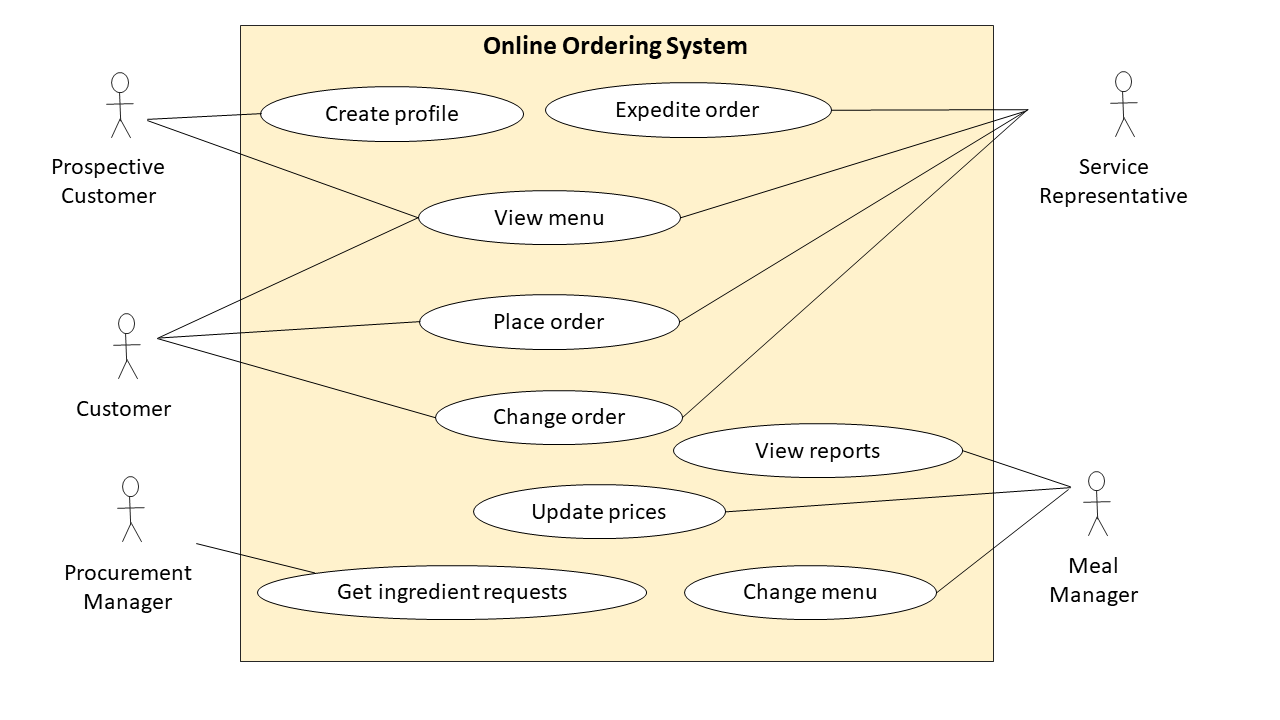
\includegraphics[width=15cm]{assets/use-case-example.png}
        \caption{Example use case diagram}
        \label{fig:use_case_example}
    \end{figure}
    \FloatBarrier

    \subsection{System requirements}
    In the following we will discuss the configurations that the system must have
    in order for the software to work smoothly and efficiently.
    \subsubsection{Functional}
    In order for the user to access the main content of the website, the website
    uses an authorization system, which contains the registration and login
    processes. \\ \indent The website collects useful materials for the
    baccalaureate exam, for example exam samples, frequently asked questions and
    also connects the students with each other via the forum page. It also makes it
    possible for the students to search for specific subjects, topics and
    materials, and take quizzes of specific materials. \\ \indent These materials
    are stored in a database from which the website gets the data, and to which it
    sends new information about the addition, deletion or modification of the
    content. \\ \indent The Welcome page contains a brief introduction about the
    website and also options to either log in or register to it. On the website we
    can access the main subjects such as Mathematics, Informatics, Romanian
    language, Hungarian language, English language, History and Geography. \\
    \indent For each subject we can access different topics. For example inside the
    Mathematics subject we can find topics such as Algebra. For each topic we can
    find different materials and access each material's page individually. For
    example Algebraic Equations. For each material there are different data, such
    as texts, exam papers, images, at least one quiz etc. Besides that the product
    also provides a Forum where users can ask questions, comment to them, search
    trough them, delete their own questions and comments. \\ \indent Each user
    individually has a Profile page where they can see their own data and even
    change it, they can also toggle between light and dark theme on the website.
    Since the users have to log in to be able to access the contents they can also
    log out from the site. \\ \indent In order to access the materials, each user
    has to have an email with which they register to the site, thus they also have
    to have a password, so when logging in they have to use the specific email and
    specific password which they used when registering. \\ \indent To ensure the
    optimal performance and user experience of the website's frontend,
    comprehensive testing with Lighthouse will be conducted. Lighthouse, integrated
    into Chrome DevTools, will assess various aspects such as performance,
    accessibility, best practices, and SEO. The testing process will involve
    evaluating scores and addressing performance challenges arising from
    unoptimized React code. Notably, Progressive Web App (PWA) features will be
    examined, even though they might not be available during testing. \\ \indent
    For the robustness and reliability of the backend, a systematic approach to
    testing will be employed through unit tests. These tests will focus on
    individual components and functions within the backend, ensuring that each unit
    of code operates as expected. Unit tests play a crucial role in validating the
    correctness of the backend functionalities, providing a solid foundation for
    the overall stability and performance of the system. Continuous integration
    practices will be implemented to automate the execution of these unit tests,
    promoting efficiency in the development process.
    \subsubsection{Non-Functional Requirements}

    \paragraph{Minimum System Requirements} \mbox{} \\ \indent
    In order to access the Example Project website, users must have a device with internet access and meet the specified platform requirements. It is essential to have an up-to-date browser installed on the device for seamless navigation and interaction with the website.

    \paragraph{Platform Requirements} \mbox{} \\ \indent
    The Example Project website is designed to operate on devices with the following minimum specifications:

    \begin{itemize}
        \item \textbf{Mobile Devices:} Android 10 or later for Android-based phones and tablets, and iOS 13 or later for Apple devices.
        \item \textbf{Computers:} Windows 10 or later, MacOS Catalina or later, or any GNU/Linux distribution with at least a Long-Term Support (LTS) kernel.
    \end{itemize}

    \paragraph{Browser Compatibility} \mbox{} \\ \indent
    The Example Project website is optimized for use with browsers based on Chromium or Firefox. Users are encouraged to access the site through up-to-date versions of these browsers for an optimal experience.

    \paragraph{Authentication Process} \mbox{} \\ \indent
    To access the Example Project website, users must authenticate themselves. The authentication process involves sending user-entered data to the backend, which then verifies the information against the database. This ensures secure and authorized access to the platform.

    \paragraph{Product Properties} \mbox{} \\ \indent
    Example Project is a user-friendly website designed to provide efficient assistance to students. It incorporates features that enhance usability, reliability, scalability, and performance.

    \paragraph{Developer and Tech Expert Specifications} \mbox{} \\ \indent
    Certain aspects of the website, such as performance, usability, and security, will be defined by developers and tech experts. These specifications will be thoroughly tested after functional testing to ensure the robustness and reliability of the system.

    \paragraph{Testing Procedures} \mbox{} \\ \indent
    The Example Project website will undergo a comprehensive testing process, including functional testing followed by performance, usability, reliability, and scalability testing. Security testing will be conducted to identify and address potential vulnerabilities.

    \paragraph{Optional but Desirable Features} \mbox{} \\ \indent
    Additional features that are not mandatory but desirable for future improvements will be identified during the development process. These may include enhancements to user interface design, additional functionalities, or integration with external systems.

    \newpage
    \section{Planning}
    \subsection{Brainstorming}
    \begin{figure}[h]
        \centering
        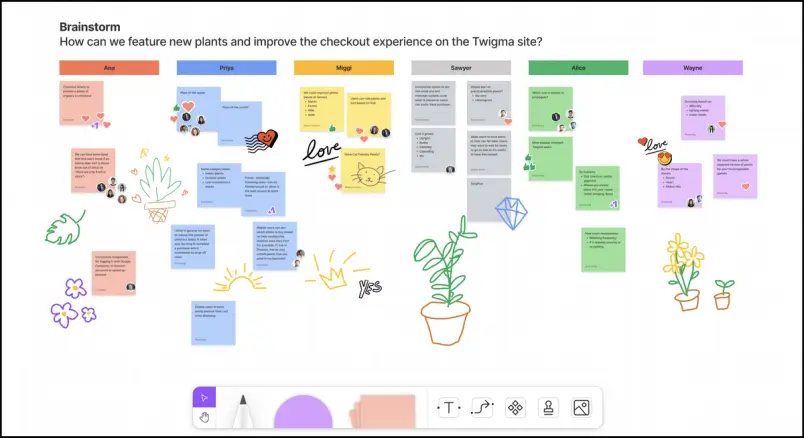
\includegraphics[width=13cm]{assets/brainstorming-example.png}
        \caption{Example of Figjam brainstorming}
        \label{fig:figjam-brainstorming}
    \end{figure}
    \FloatBarrier

    \begin{figure}[h]
        \centering
        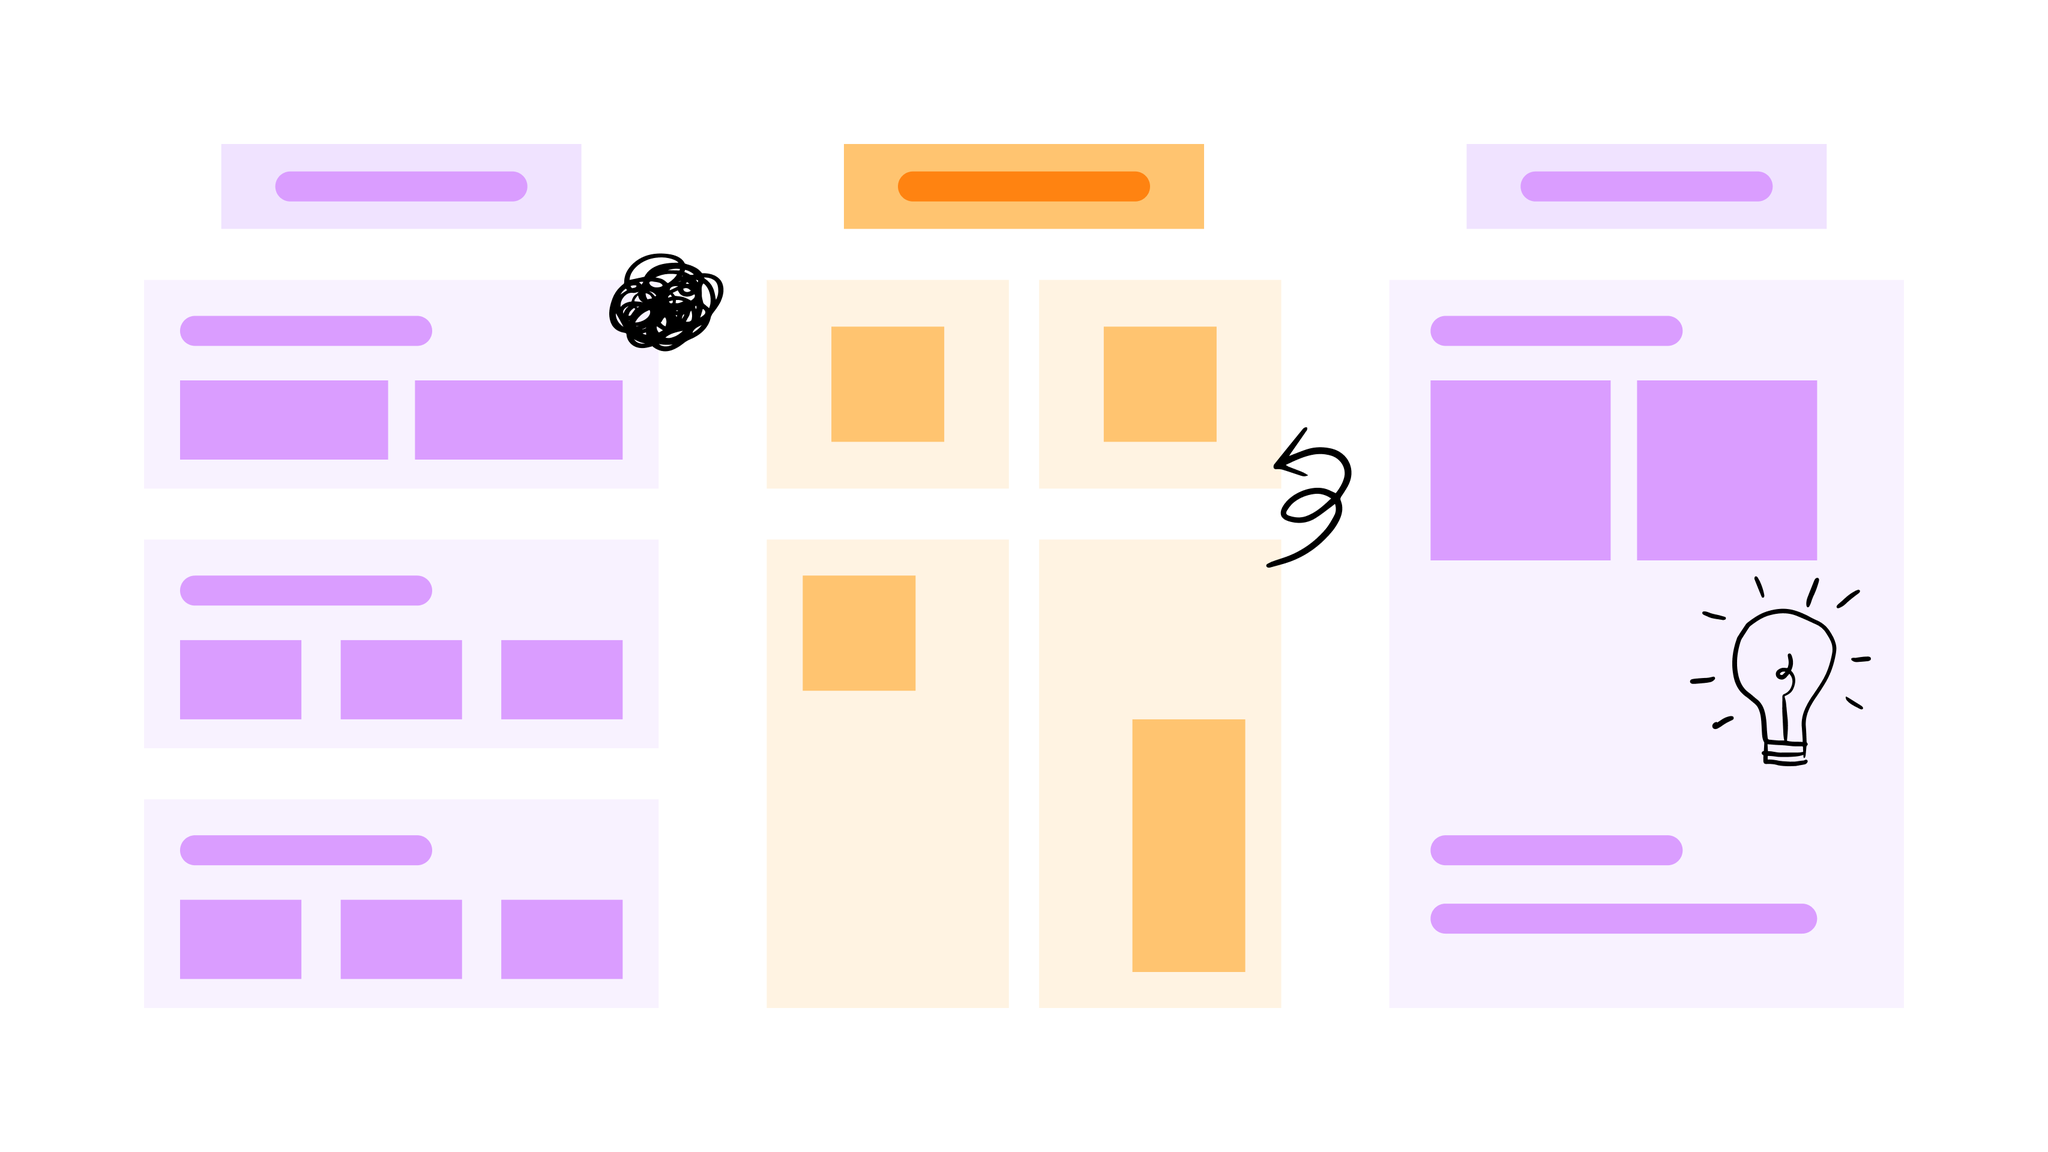
\includegraphics[width=15cm]{assets/another-brainstorming-example.png}
        \caption{Another example of Figjam brainstorming}
        \label{fig:figjam-overview}
    \end{figure}
    \FloatBarrier

    We started our planning by brainstorming our ideas in a Figjam project
    (\autoref{fig:figjam-brainstorming}). Later on this Figjam project grow out
    (\autoref{fig:figjam-overview}) and it helped developing the project
    architecture (\autoref{subseq:architecture}), the wireframe and the design
    (\autoref{subseq:wireframe-and-design}).

    \newpage
    \subsection{Architecture}\label{subseq:architecture}

    \begin{figure}[h]
        \centering
        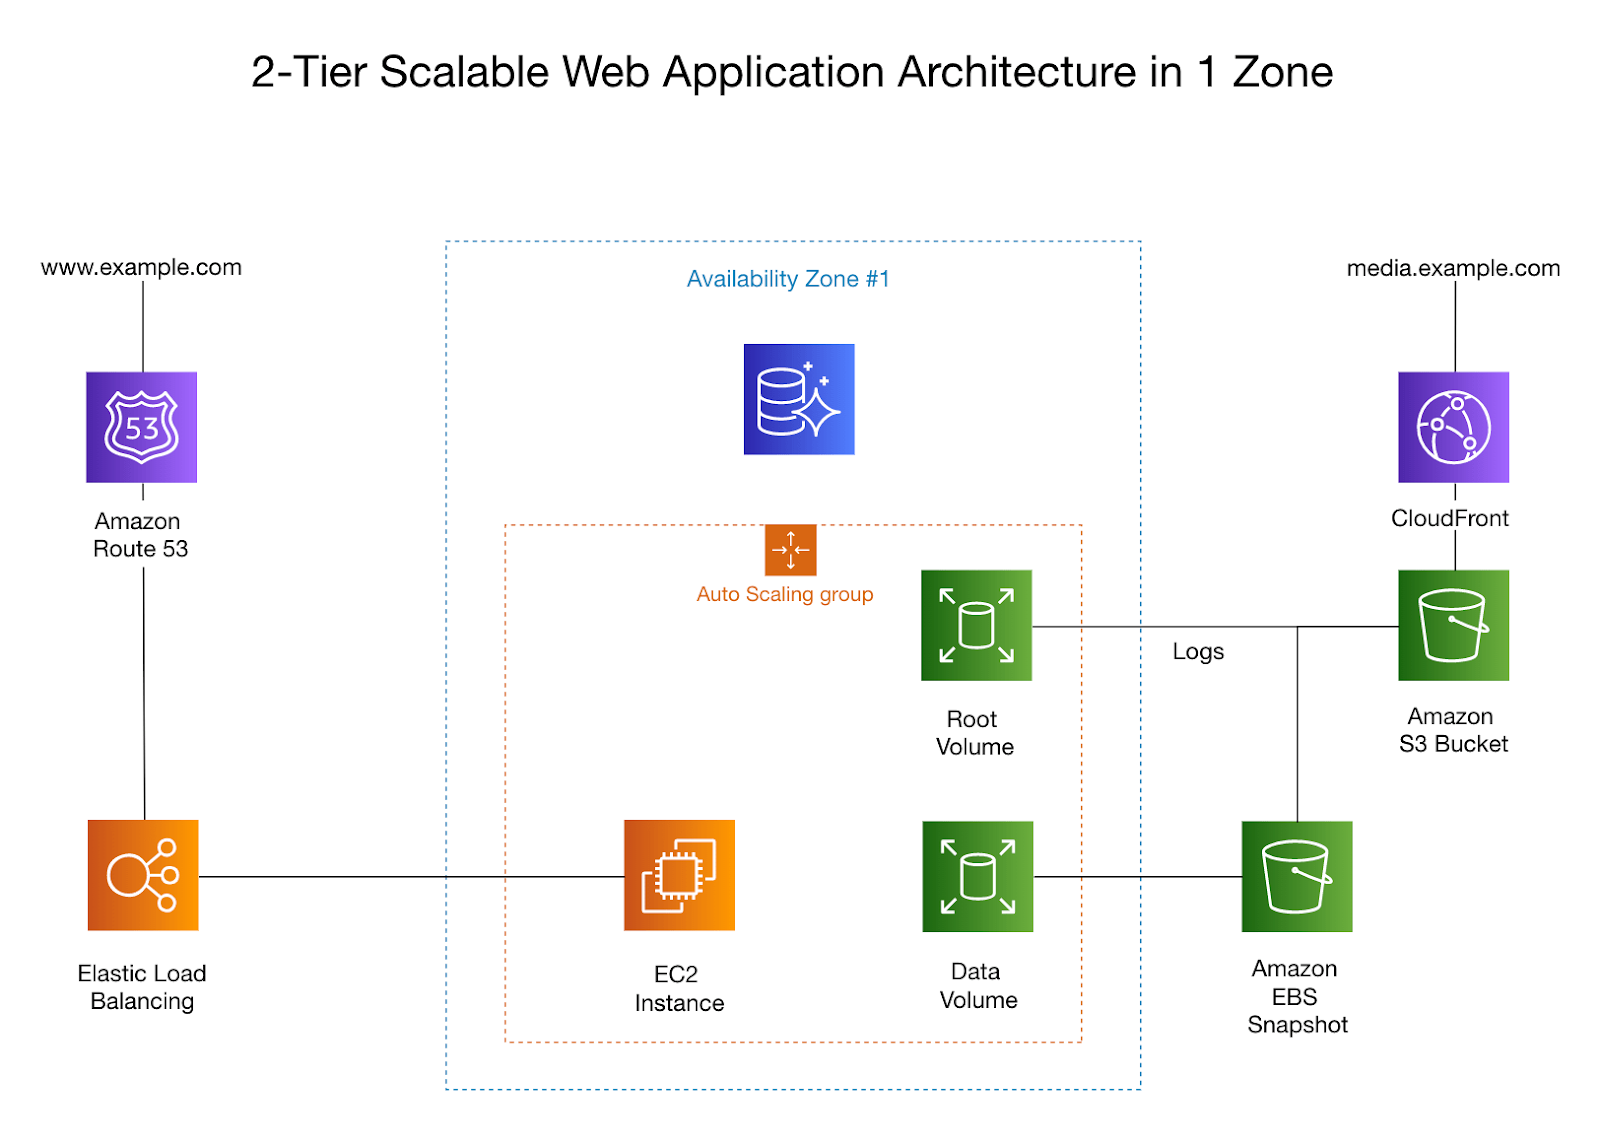
\includegraphics[width=16cm]{assets/architecture-example.png}
        \caption{Example Project Architecture}
        \label{fig:architecture}
    \end{figure}
    \FloatBarrier

    When we began planning the application's architecture, we considered it's
    future and the requirements it needed to fulfill. (\autoref{fig:architecture})

    \subsubsection{Database}
    As mentioned earlier in this subsection, our focus was on anticipating the
    future needs of the application. We aimed to establish a robust foundation
    capable of supporting a forum for asking and answering questions. For efficient
    database management without compromising application stability, we opted for
    the reliable PostgreSQL system. Beyond meeting our immediate needs, PostgreSQL
    boasts a thriving community and numerous plugins, which will prove beneficial
    in addressing future challenges within this project.

    \subsubsection{Backend}
    When selecting the backend technology for this project, our priority was to
    find a robust and straightforward solution. While NodeJS was initially under
    consideration, we sought a framework that offered greater reliability and a
    more seamless approach to dependency management than Node.

    After thorough deliberation, we ultimately decided on Python Django. Our choice
    was influenced by its strong community support and the inclusion of valuable
    default features, such as the ORM (Object-Relational Mapping) module. Django
    provides a solid foundation for our backend, ensuring a smoother development
    process and offering a wealth of built-in functionalities.

    \subsubsection{Frontend}
    In choosing our frontend technologies, the decision was straightforward for our
    team: React with TypeScript, TailwindCSS, and the ViteJS server proved to be
    the optimal combination.

    Despite the rapid emergence of frontend web frameworks in the NodeJS ecosystem,
    React stood out as one of the most stable choices. Its stability not only
    ensured a secure development path but also provided our team with abundant
    resources whenever we needed assistance or guidance.

    The utilization of TailwindCSS facilitated the seamless implementation of our
    custom designs, making the process remarkably straightforward. Additionally,
    TypeScript played a crucial role in error prevention, significantly reducing
    the occurrence of mistakes and bugs throughout the development phase.

    \subsubsection{Documentation Generation}
    When we started implementing the project we were thinking ahead how could we
    help the team with fast technical documentation.

    After careful consideration, we opted for Python Sphinx with the Furo theme.
    Through some configuration adjustments, we successfully generated a
    high-quality, searchable technical documentation for our Django backend. While
    we have yet to implement technical documentation generation for the frontend,
    the tools in place have already proven crucial. Expanding this documentation
    generation tool to cover the frontend is a top priority for future development.

    \subsubsection{Dockerizing the architecture}
    Recognizing the challenges inherent in software development, we proactively
    adopted a Dockerized approach from the project's inception. Dockerizing the
    database, backend, frontend, and documentation generation tool provided
    distinct services, significantly easing our development workflow.

    The communication between the frontend and backend services relied on REST
    APIs, while Django's ORM facilitated the interaction between the backend and
    the database.

    The documentation generation tool, operating separately, had a copy of the
    backend during documentation generation to prevent inadvertent disruptions.

    Clients can access our project conveniently via a web browser or a Progressive
    Web App (PWA).

    \subsection{Conventions}

    To ensure a consistent development experience, our project follows several
    conventions.

    \subsubsection{Variable Naming Conventions}

    \paragraph{Backend (Django Framework)}
    For backend development, we adhere to Django Framework's naming conventions for
    variables.\footnote{
        \href{https://docs.djangoproject.com/en/dev/internals/contributing/writing-code/coding-style/}{Official
            Django Documentation}}\footnote{
        \href{https://learndjango.com/tutorials/django-best-practices-projects-vs-apps}{LearnDjango}
    }
    \paragraph{Frontend (React TypeScript)} Frontend development follows React
    TypeScript's variable naming conventions.\footnote{
        \href{https://levelup.gitconnected.com/managing-types-in-react-typescript-the-right-way-fa1ecc50a2bf}{Medium}
    }

    \textbf{Some examples:}
    \begin{itemize}
        \item PascalCase is used for type names.
        \item Avoid using the "I" prefix for interfaces.
        \item Utilize the \_ prefix for private properties.
        \item Maintain consistent naming for component props types (e.g., \texttt{type
                  CustomComponentProps}).
    \end{itemize}

    \subsubsection{Sprint and Task Management}\label{subseq:conventions-sprint-and-task-managment}

    Later, in subsequent sections, we will explore our use of
    \href{https://trello.com/}{Trello} for sprint management
    (\autoref{subseq:lean-and-trello}), GitHub (Git) for version control
    (\autoref{subseq:version-control}), and the management of smaller tasks through
    GitHub issues (\autoref{subseq:task-managment-github-issue}).

    \paragraph{Branch Naming Convention}
    \begin{itemize}
        \item Start the branch name with the GitHub issue number.
        \item After the issue number, use the issue title in lowercase separated with the "-"
              symbol.
        \item Example: \texttt{13-login-system} for GitHub issue \#13 titled "Login system."
    \end{itemize}

    \paragraph{Commits}
    \begin{enumerate}
        \item Use \href{https://www.conventionalcommits.org/en/v1.0.0/}{Conventional Commits}
              for all commits.
        \item Format: \texttt{<type>[optional scope]: <description>}
        \item Types:
              \begin{itemize}
                  \item \texttt{fix}: Bugfixes, code fixes.
                  \item \texttt{feat}: Feature implementation.
                  \item \texttt{chore}: Code cleanup.
              \end{itemize}
        \item Example: \texttt{feat(api)!: send an email to the customer when a product is
                  shipped}
              \begin{itemize}
                  \item The "!" flag is optional and indicates breaking changes.
              \end{itemize}
    \end{enumerate}

    \paragraph{Pull Requests} \mbox{} \\ \indent
    When submitting changes via pull request, reference the relevant GitHub issue. Ensure that the pull request includes a clear and concise description of the changes.

    \subsection{System Overview: UML, Backend Modules, and Personas}
    Add diagrams about the overview of your project, like UML, Backend Modules,
    Class and Persona diagrams. \\ \textbf{Do's:}
    \begin{itemize}
        \item clear and simplistic images
        \item digitally created images are better, but you can also use hand drawn diagrams
        \item show the main content
        \item easy to read diagrams
        \item instead of empty spaces use bigger fonts or structure your diagram better
    \end{itemize}
    \textbf{Don'ts:}
    \begin{itemize}
        \item images with black background (\autoref{fig:backend-uml})
        \item too big images (\autoref{fig:backend-modules})
        \item blurry or pixeled images --- even you can't see clearly what it really is about
        \item if you have big images show them at the appendix part, although that's not
              really part of the documentation, so include necessary parts of the big image
              here
        \item do not add everything in one image, if you have multiple parts that you want to
              include separate them by context, style or importance
    \end{itemize}

    Good examples are \autoref{fig:class-diagram} for class diagrams and
    \autoref{fig:persona-diagram} for persona diagrams. Bad examples are
    \autoref{fig:backend-uml} for not clear images with black background and
    \autoref{fig:backend-modules} for too big images with small fonts and complex
    composition.
    \begin{figure}[H]
        \centering
        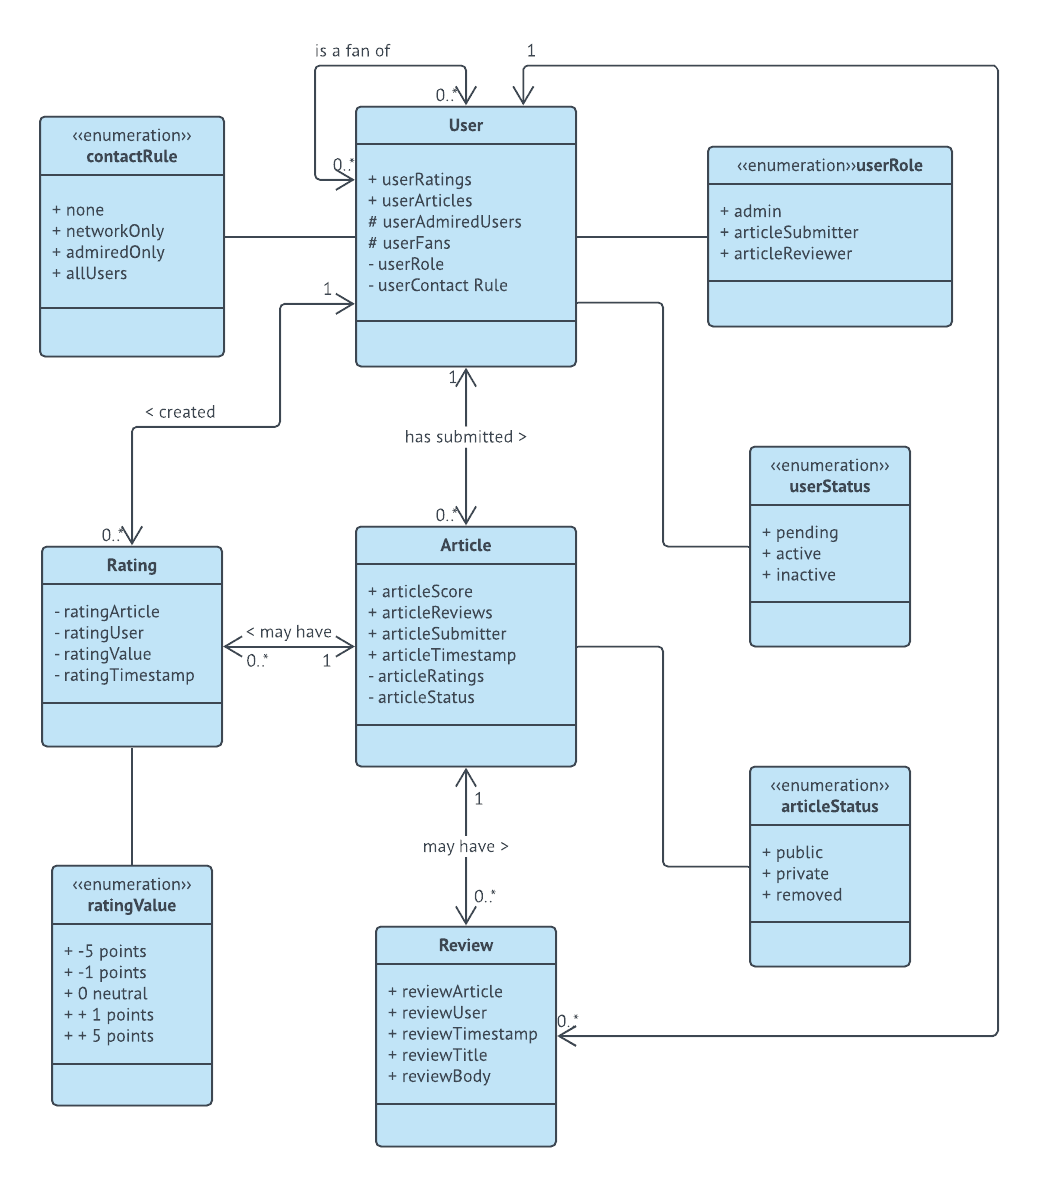
\includegraphics[width=1\linewidth]{assets/class_diagram.png}
        \caption{Class diagram}
        \label{fig:class-diagram}
    \end{figure}
    \FloatBarrier

    \begin{figure}[H]
        \centering
        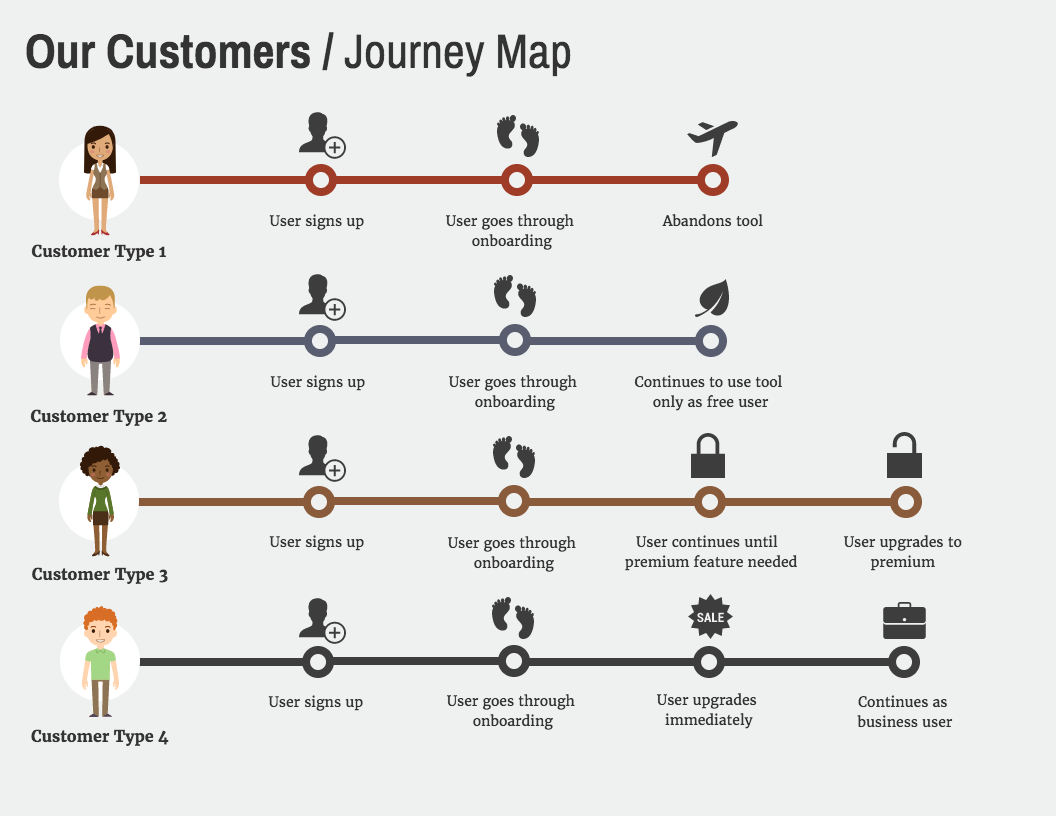
\includegraphics[width=1\linewidth]{assets/persona-diagram-example.png}
        \caption{Example Persona diagram}
        \label{fig:persona-diagram}
    \end{figure}
    \FloatBarrier

    \begin{figure}[H]
        \centering
        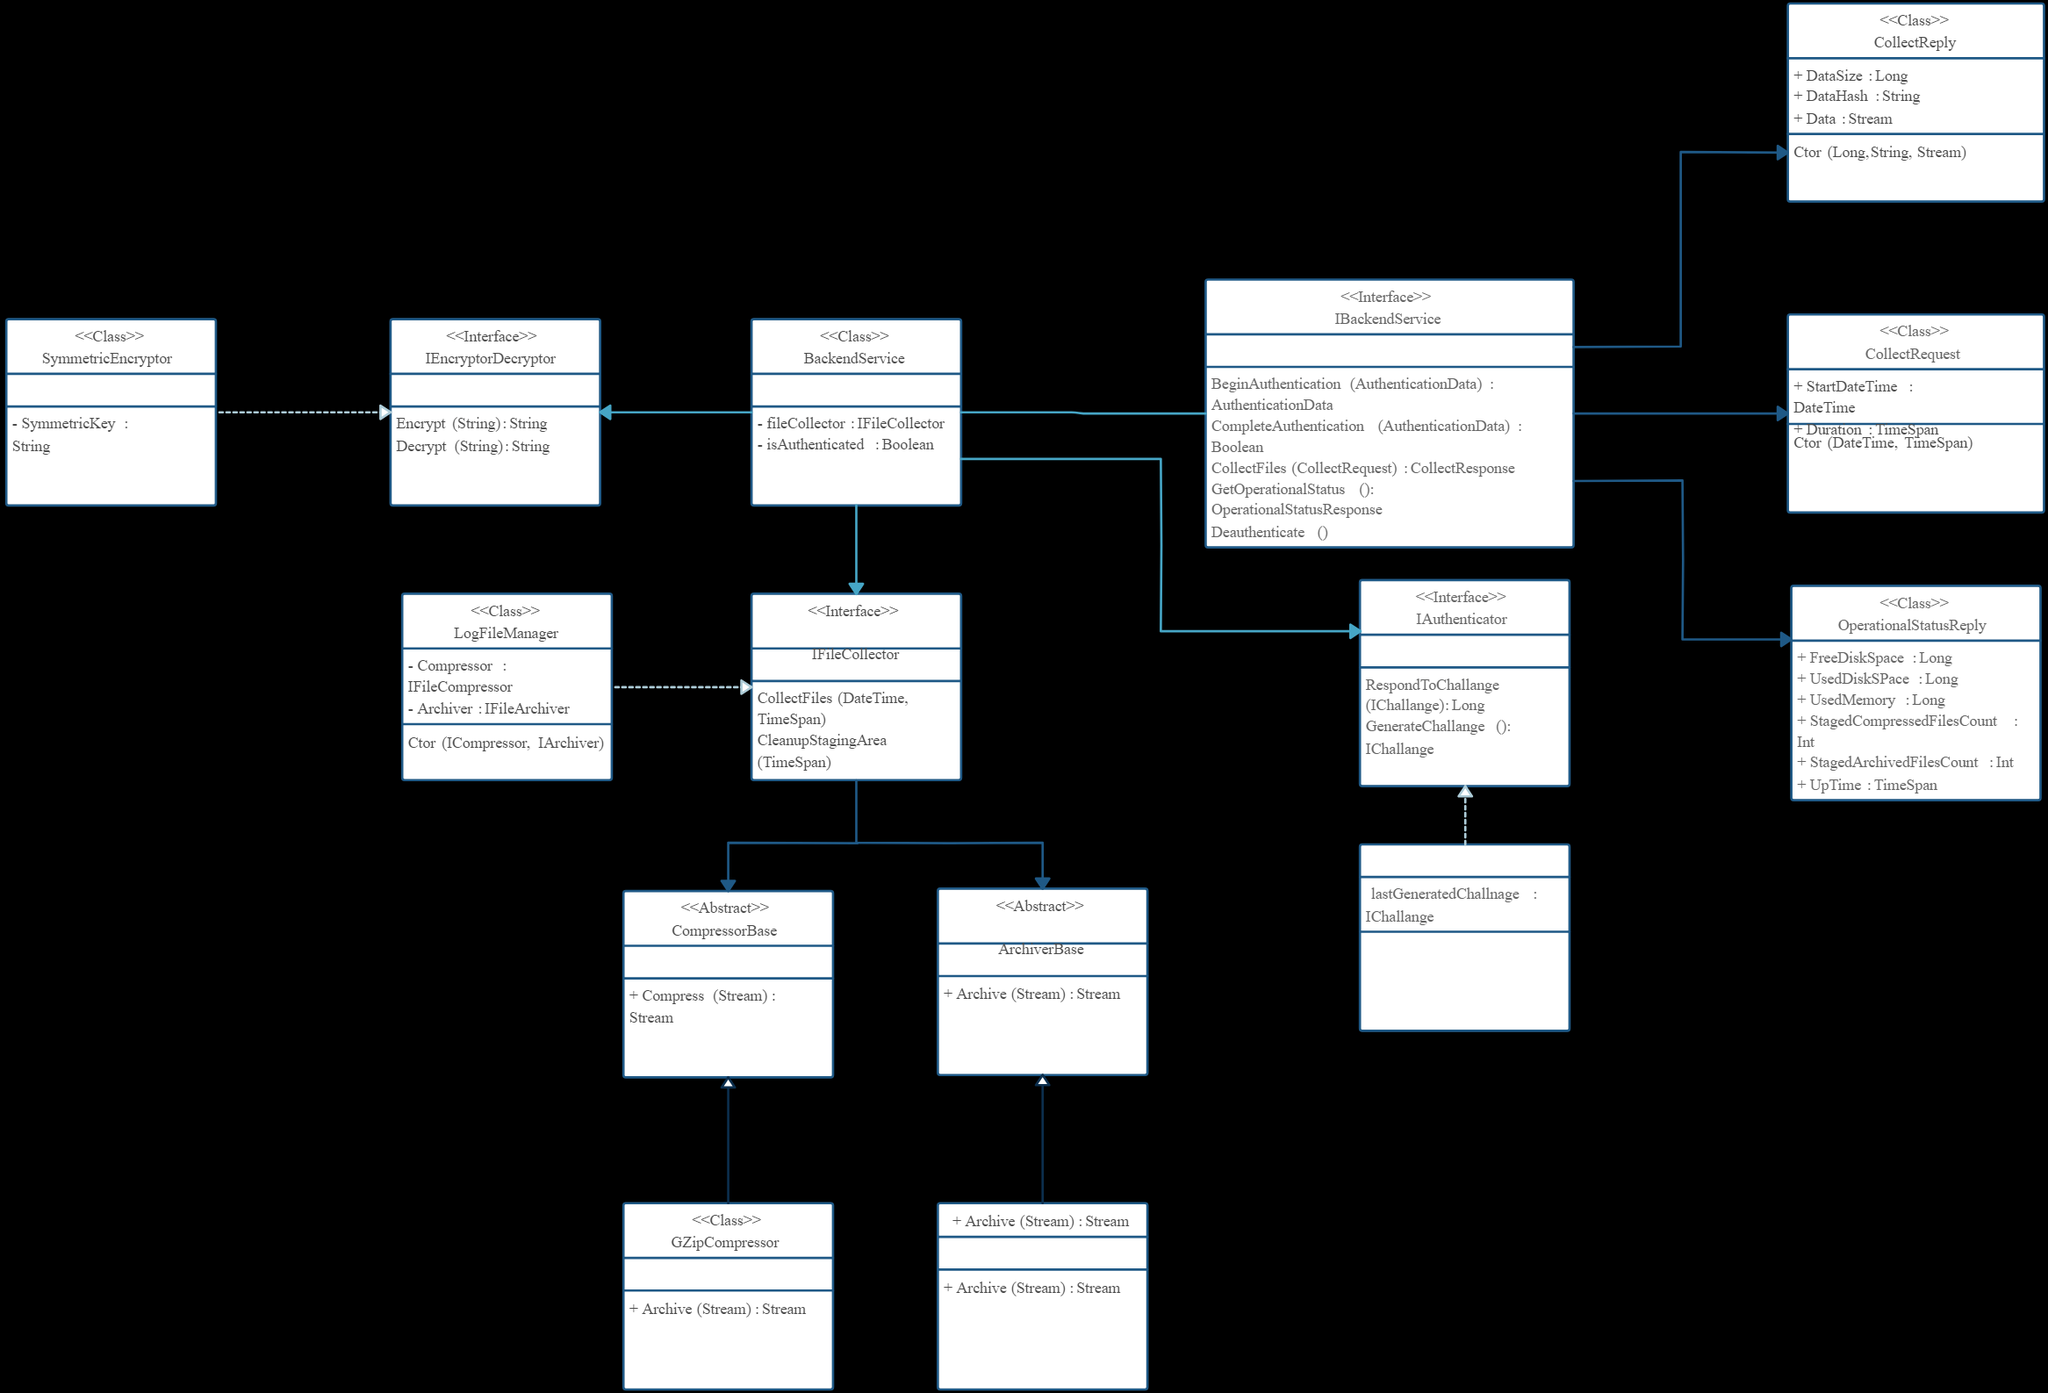
\includegraphics[width=1\linewidth]{assets/backend-uml-example.png}
        \caption{Example UML diagram of the backend}
        \label{fig:backend-uml}
    \end{figure}
    \FloatBarrier

    \begin{figure}[H]
        \centering
        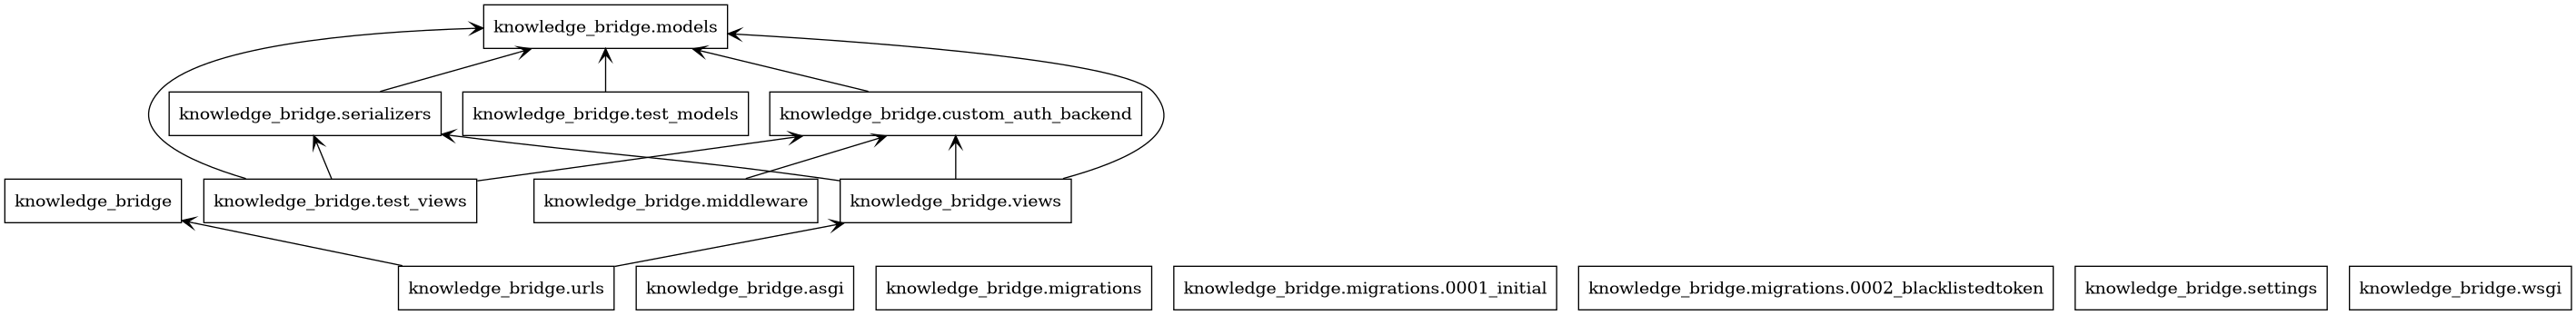
\includegraphics[width=1\linewidth]{assets/KnowledgeBridgePackages.png}
        \caption{Diagram of the backend modules}
        \label{fig:backend-modules}
    \end{figure}
    \FloatBarrier

    \newpage
    \subsection{Wireframe and Design (UX \& UI)}\label{subseq:wireframe-and-design}
    \subsubsection{Wireframe}
    \begin{figure}[h]
        \centering
        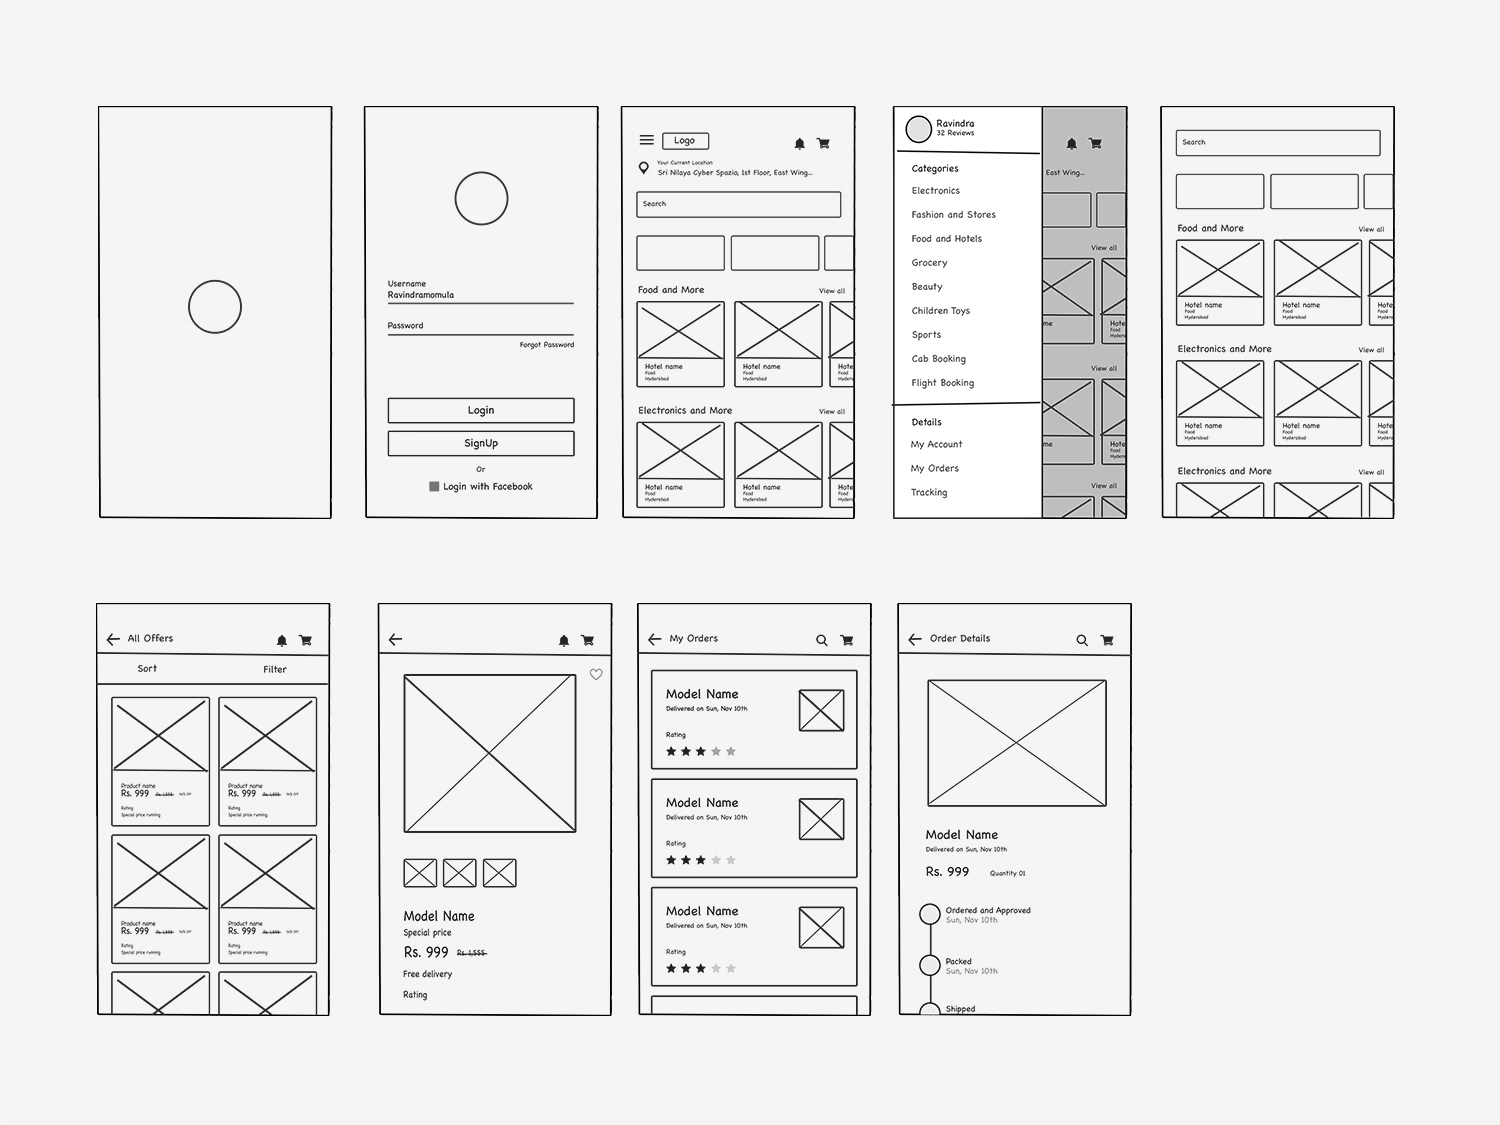
\includegraphics[width=1\linewidth]{assets/wireframe-example.png}
        \caption{Example Wireframe overview}
    \end{figure}
    \FloatBarrier

    \newpage
    \subsubsection{Design}
    The overall design was created using FigJam and Figma. The wireframe was made
    in FigJam and based on that the mockup was made in Figma.

    \begin{figure}[H]
        \centering
        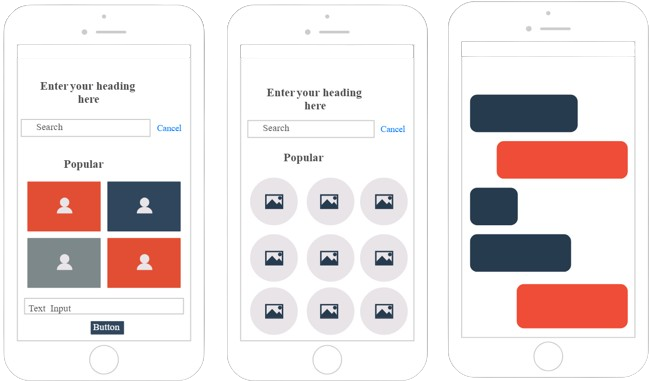
\includegraphics[width=1\linewidth]{assets/mockup-example.png}
        \caption{Example mockup overview}
    \end{figure}
    \FloatBarrier

    \begin{figure}[H]
        \centering
        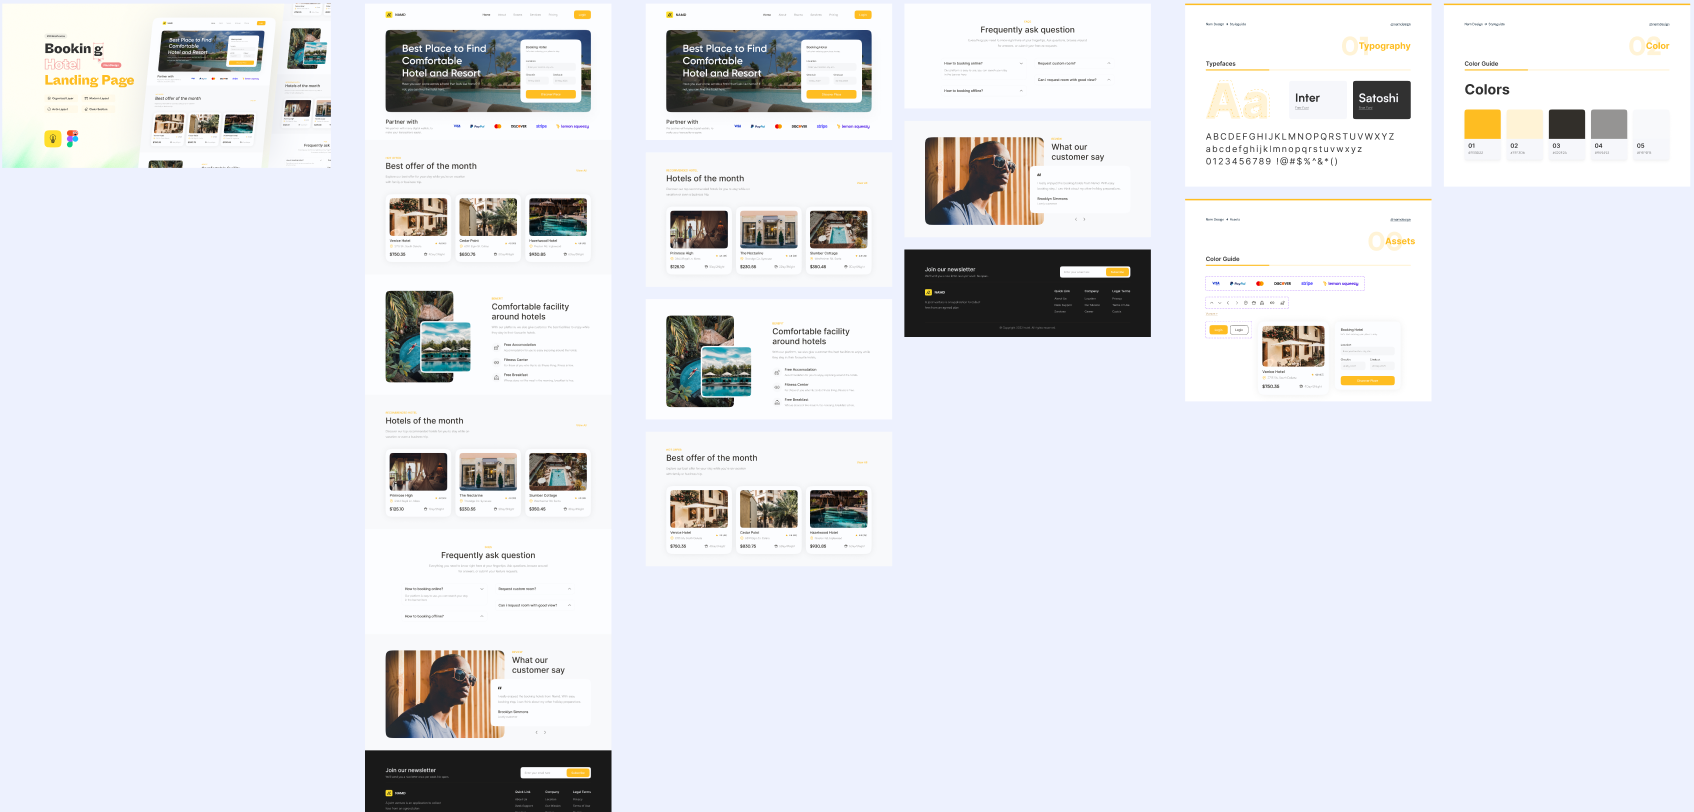
\includegraphics[width=1\linewidth]{assets/design-overview-example.png}
        \caption{Example Design overview}
    \end{figure}
    \FloatBarrier

    \newpage
    The Welcome page is the first page that anyone can see who accesses the website. From here the Registration page and Login page is accessible by clicking the corresponding buttons, for the registration either the "Register" button or the "Get started here button" and for the login the "Login" button.

    \begin{figure}[H]
        \centering
        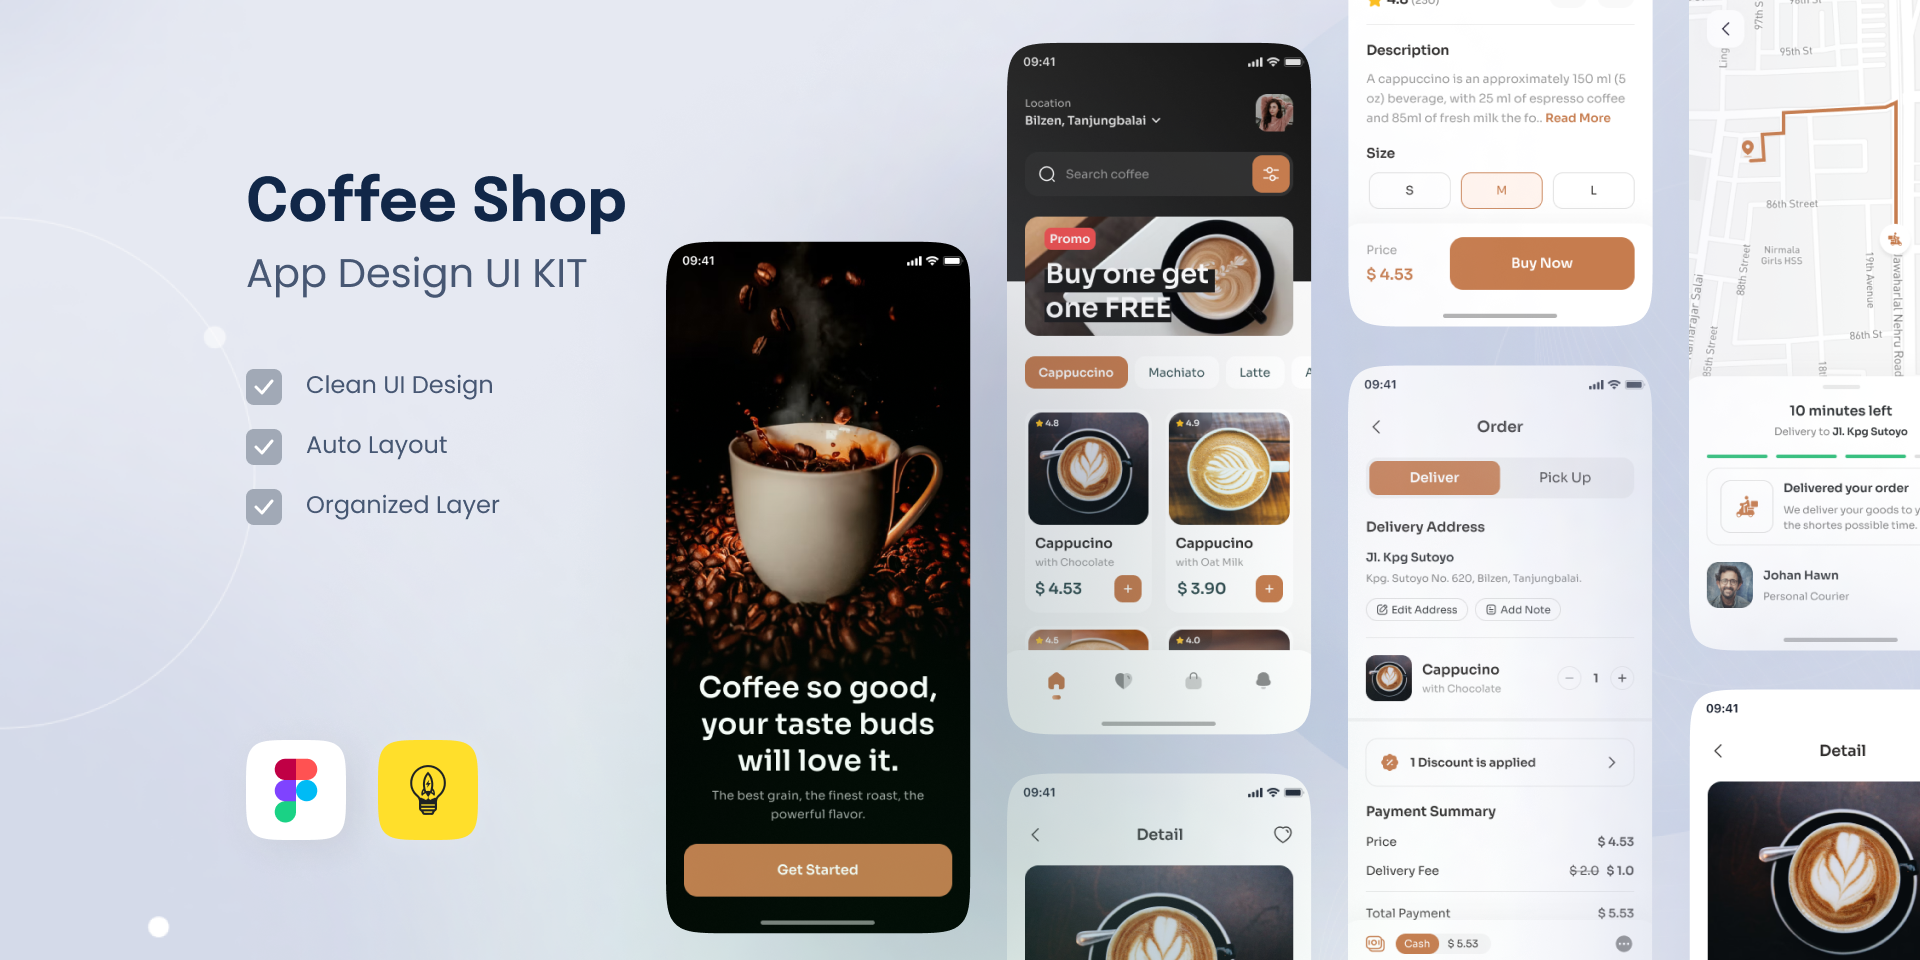
\includegraphics[width=0.6\linewidth]{assets/mobile-design-example.png}
        \caption{Example Mobile Design overview}
    \end{figure}
    \FloatBarrier

    On the Registration page the user can choose their authentification type,
    either student or teacher, enter their email and their password and register
    via the "Register" button if every detail is correct. If they already have an
    account they can go to the Login page from here as well. The page also contains
    the logo.

    \begin{figure}[H]
        \centering
        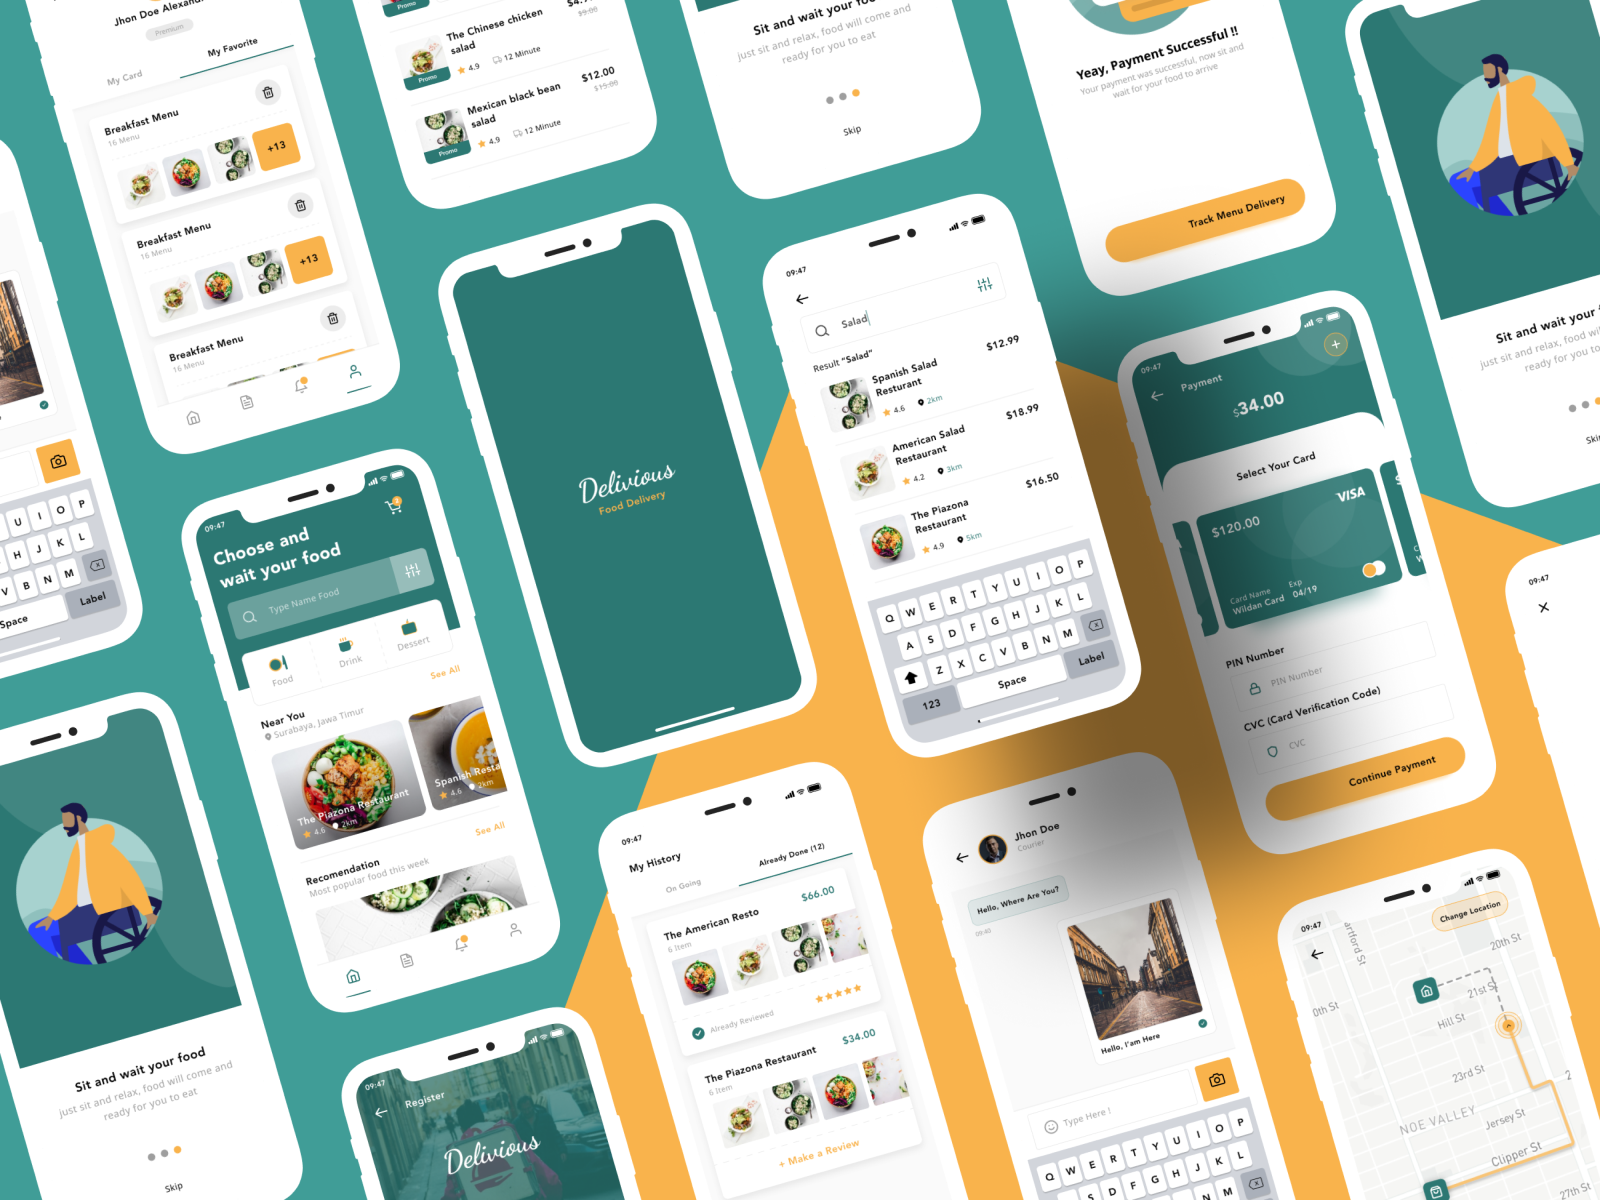
\includegraphics[width=0.6\linewidth]{assets/another-design-example.png}
        \caption{Another Example Design overview}
    \end{figure}
    \FloatBarrier

    On the Login page the user can enter thier email and password and log in via
    the "Login" button, or go to the Register page if they do not have an account
    yet. The page also contains the logo. \newpage

    \subsection{Database plan}
    \begin{figure}[h]
        \centering
        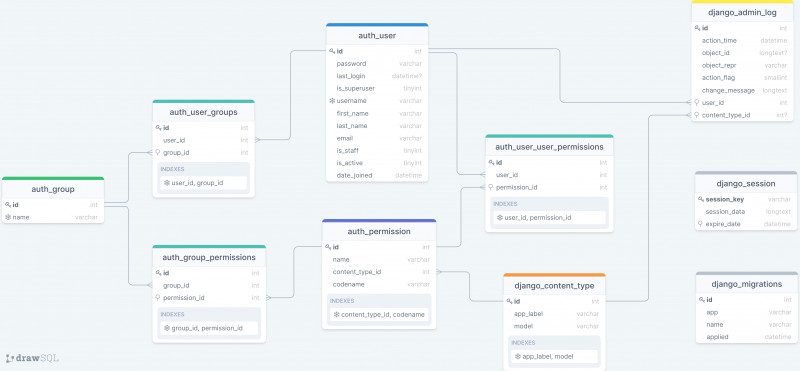
\includegraphics[width=16cm]{assets/database-diagram-example.jpg}
        \caption{Example database diagram}
        \label{fig:database-diagram}
    \end{figure}
    \FloatBarrier

    \subsection{Lean Metodology and Sprint Managment with Trello}\label{subseq:lean-and-trello}

    Here you can see an example about the Task and Sprint Managment with
    \href{https://trello.com/}{Trello}. You may use any other task managing tool,
    for example \href{https://github.com/features/issues}{GitHub issues} (see
    specific example belove), \href{https://www.notion.so/}{Notion},
    \href{https://www.atlassian.com/software/jira}{Jira},
    \href{https://www.dragapp.com/blog/free-task-management-software/}{etc.}

    \begin{figure}[h]
        \centering
        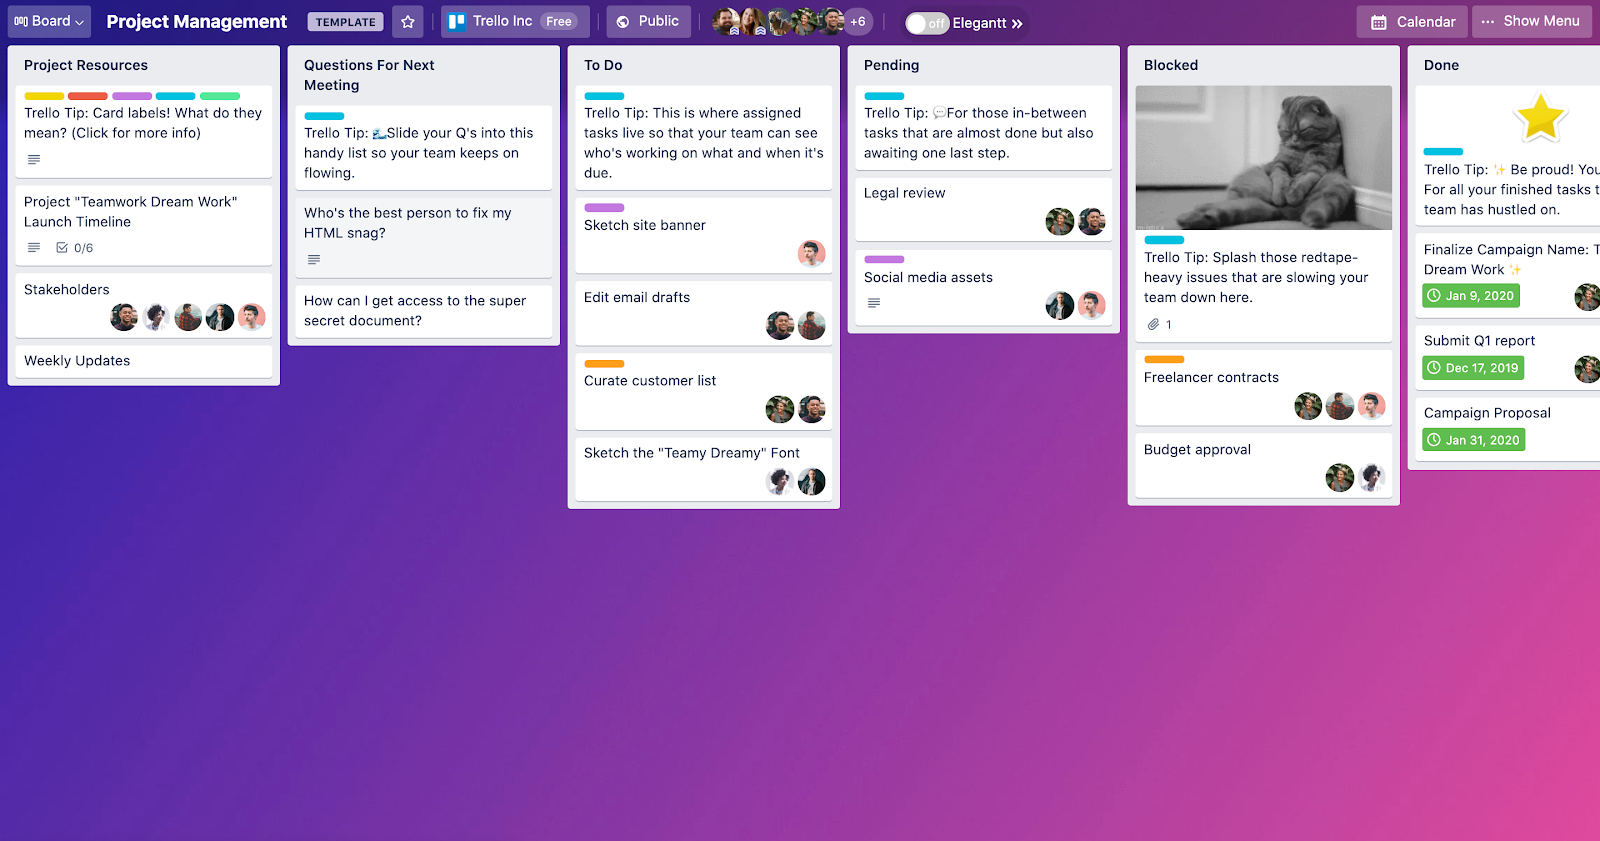
\includegraphics[width=14cm]{assets/trello-board-example.png}
        \caption{Example Trello board}
        \label{fig:trello-board}
    \end{figure}
    \FloatBarrier

    \begin{figure}[H]
        \centering
        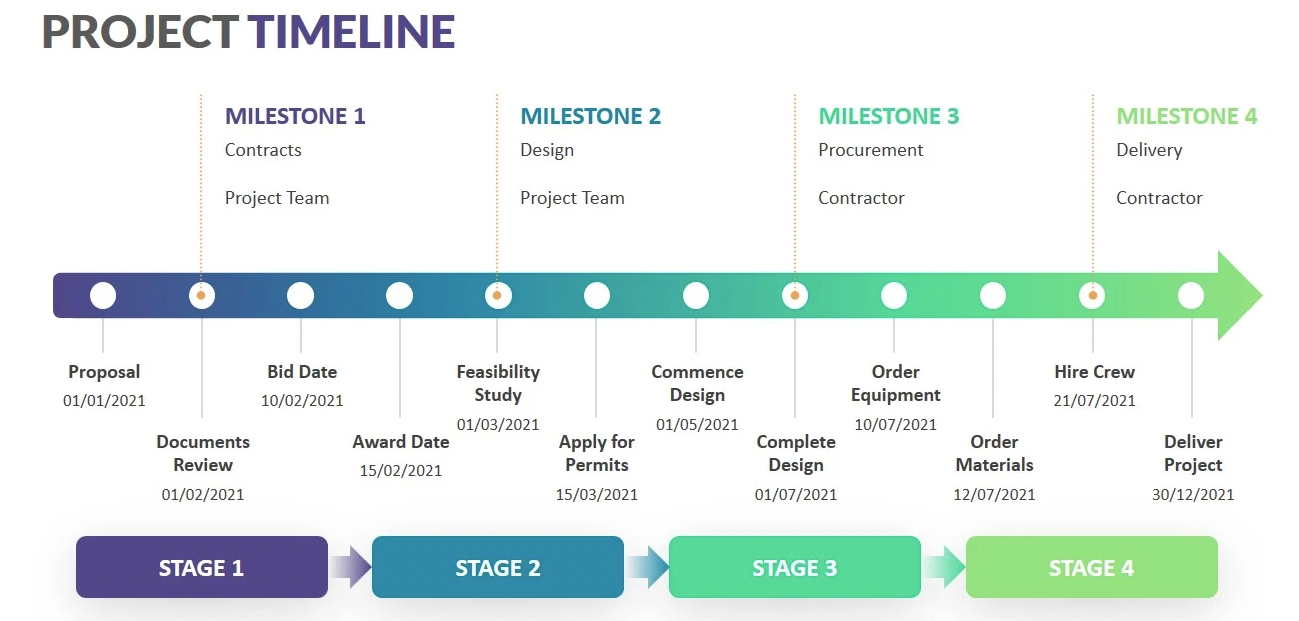
\includegraphics[width=16cm]{assets/project-timeline-example.png}
        \caption{Example Project Timeline}
        \label{fig:project-timeline}
    \end{figure}
    \FloatBarrier

    Given our small team size, the Lean methodology proved more suitable than Agile
    for our fast-paced development needs. We adopted a weekly sprint model to
    maintain an efficient workflow (\autoref{fig:trello-board}).

    We formulated our sprints based on a predefined project timeline, as visualized
    in \autoref{fig:project-timeline}.

    The Trello board depicted in Figure (\autoref{fig:trello-board}) illustrates
    the five states of our sprint management process:
    \begin{itemize}
        \item \textbf{Backlog State:}
              This state served as the repository for sprint drafts and ideas.

        \item \textbf{To-Do State:}
              Tasks slated for upcoming sprints were organized here.

        \item \textbf{Doing State:}
              Active sprints, representing tasks actively in progress, were managed in this state.

        \item \textbf{Blocked State:}
              Tasks encountering obstacles preventing completion found their place here.

        \item \textbf{Waiting for Approval State:}
              Sprints requiring review and approval were designated to this state.

        \item \textbf{Done State:}
              Successfully completed sprints were archived in this final state.

    \end{itemize}

    Trello facilitated seamless sprint management, offering the ability to provide
    details and engage in discussions about specific sprints, as demonstrated in
    Figure (\ref{fig:trello-task-example}).

    \begin{figure}[H]
        \centering
        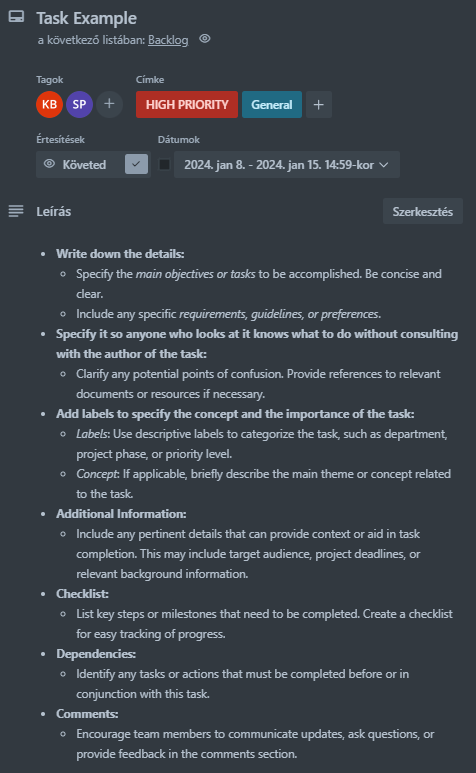
\includegraphics[width=0.7\linewidth]{assets/trello-task-example.png}
        \caption{Example Trello task}
        \label{fig:trello-task-example}%
    \end{figure}
    \FloatBarrier

    \subsection{Task Managment with Github issues}\label{subseq:task-managment-github-issue}

    Here you can see an example about using GitHub issues as a task management
    tool. You may use other task managing tools.

    Task Management with GitHub Issues As previously discussed in
    \autoref{subseq:conventions-sprint-and-task-managment}, task management is
    conducted through GitHub issues. The referenced subsection highlighted how
    adhering to conventions has seamlessly integrated GitHub issues into our
    development workflow, providing an efficient and organized approach to task
    management (\autoref{fig:github-issues-closed}).

    GitHub Issues proved vital for communication related to specific tasks,
    particularly when additional guidance was required (refer to
    \autoref{fig:github-issue-example}).

    \begin{figure}[h]
        \centering
        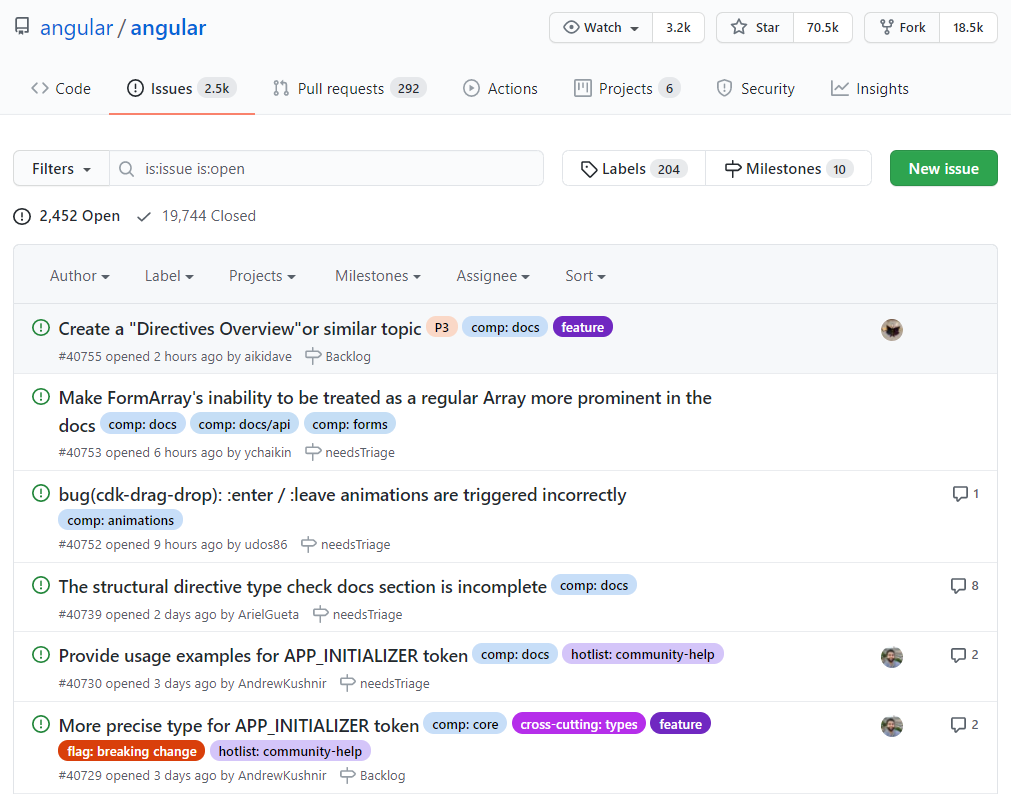
\includegraphics[width=16cm]{assets/github-issue-overview-example.png}
        \caption{Example of Github Issues Overview}
        \label{fig:github-issues-closed}
    \end{figure}
    \FloatBarrier

    \begin{figure}[h]
        \centering
        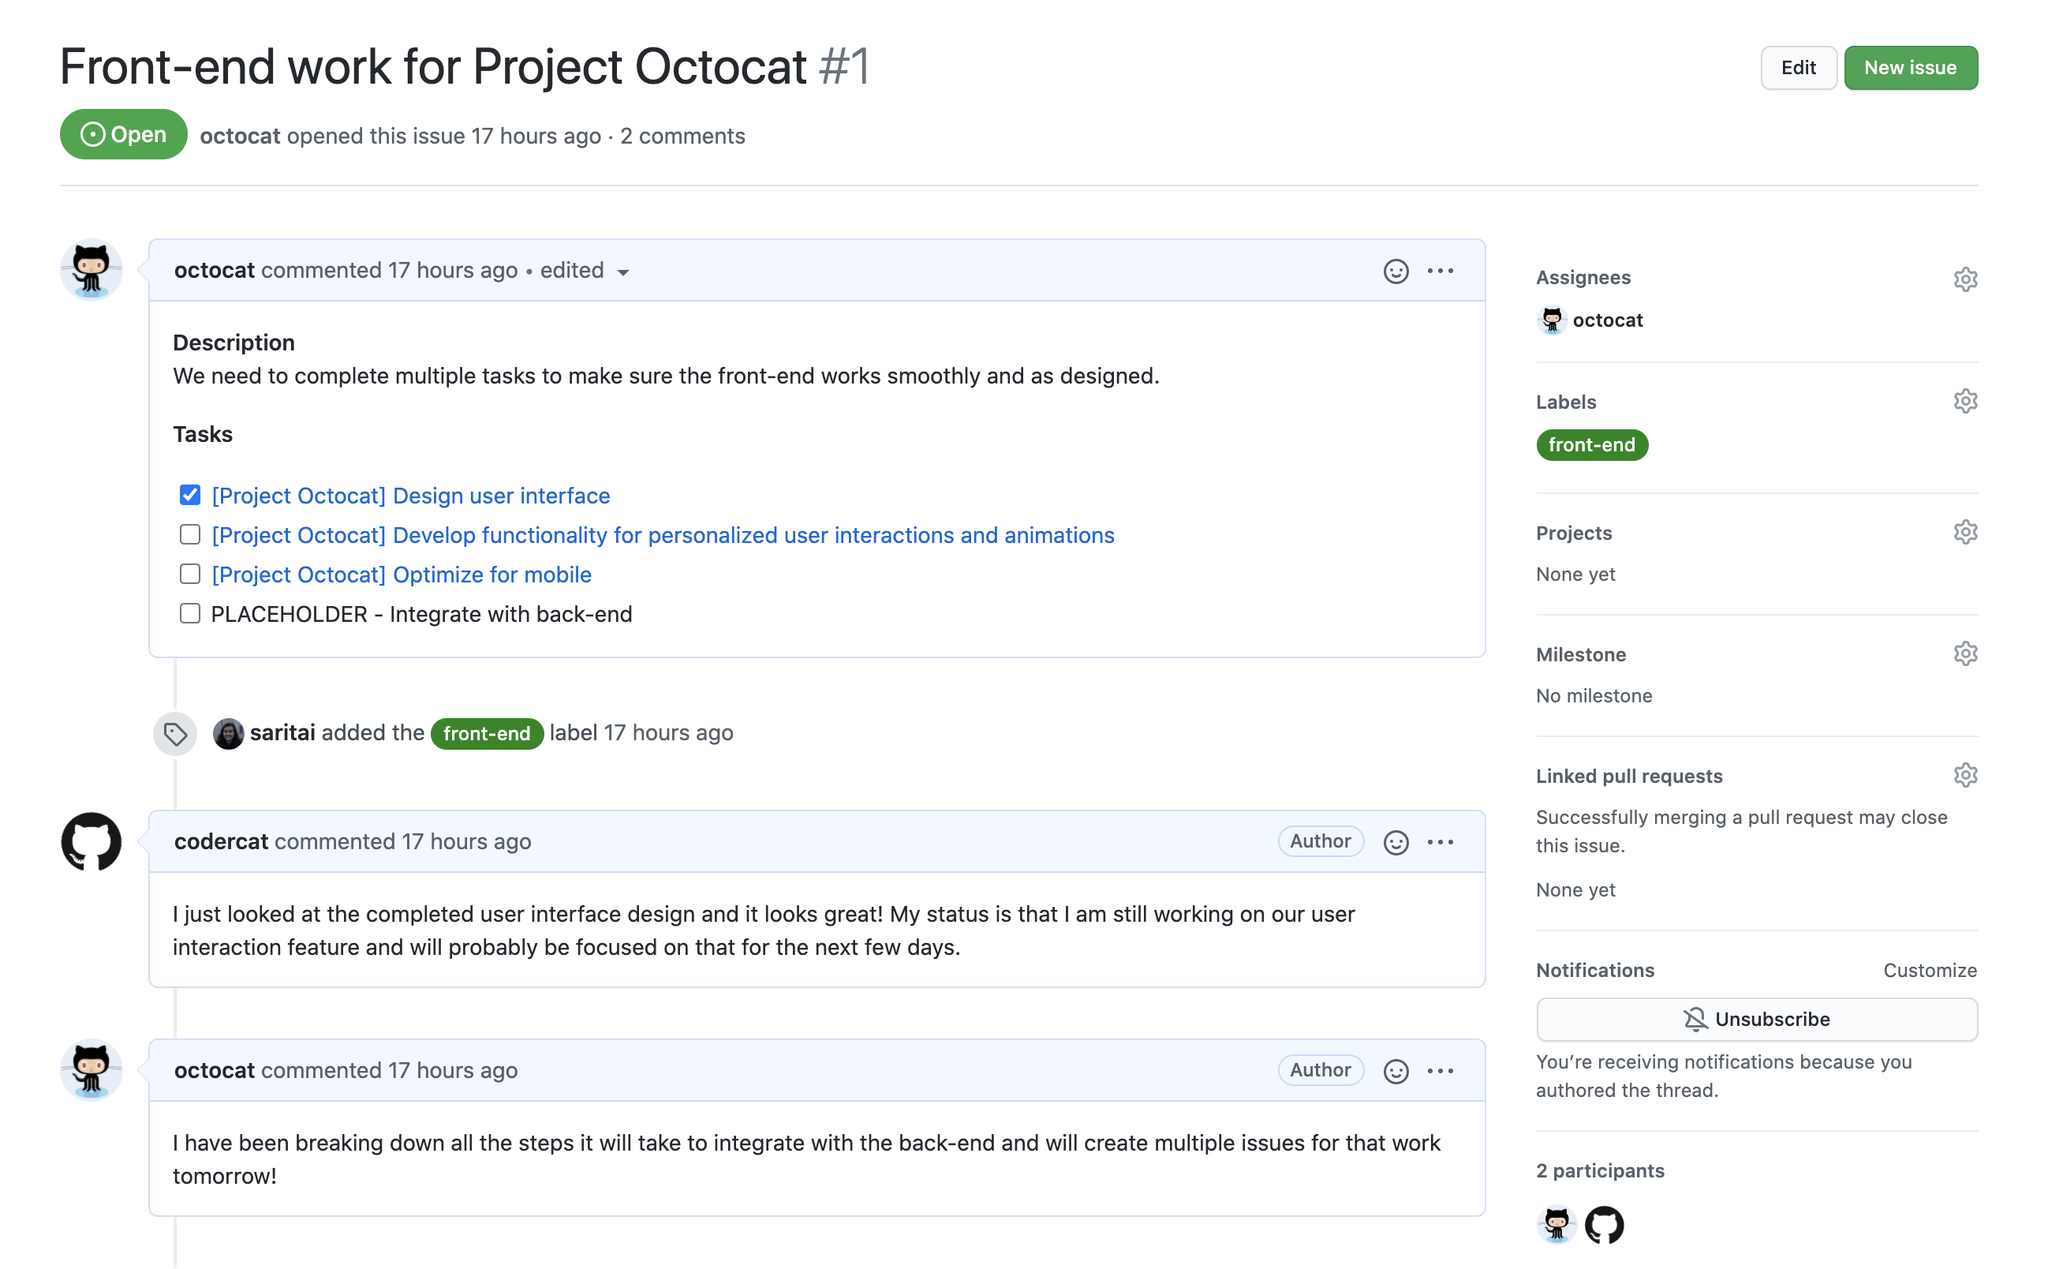
\includegraphics[width=16cm]{assets/github-issue-example.png}
        \caption{Example of Github Issue}
        \label{fig:github-issue-example}%
    \end{figure}
    \FloatBarrier

    \subsection{Version Control with Github}\label{subseq:version-control}

    Here is an example about version controlling with GitHub. Instead of GitHub you
    can use other version control systems based on
    \href{https://git-scm.com/}{Git}, \href{https://www.nongnu.org/cvs/}{CVS},
    \href{https://subversion.apache.org/}{SNV} etc.

    \begin{figure}[H]
        \centering
        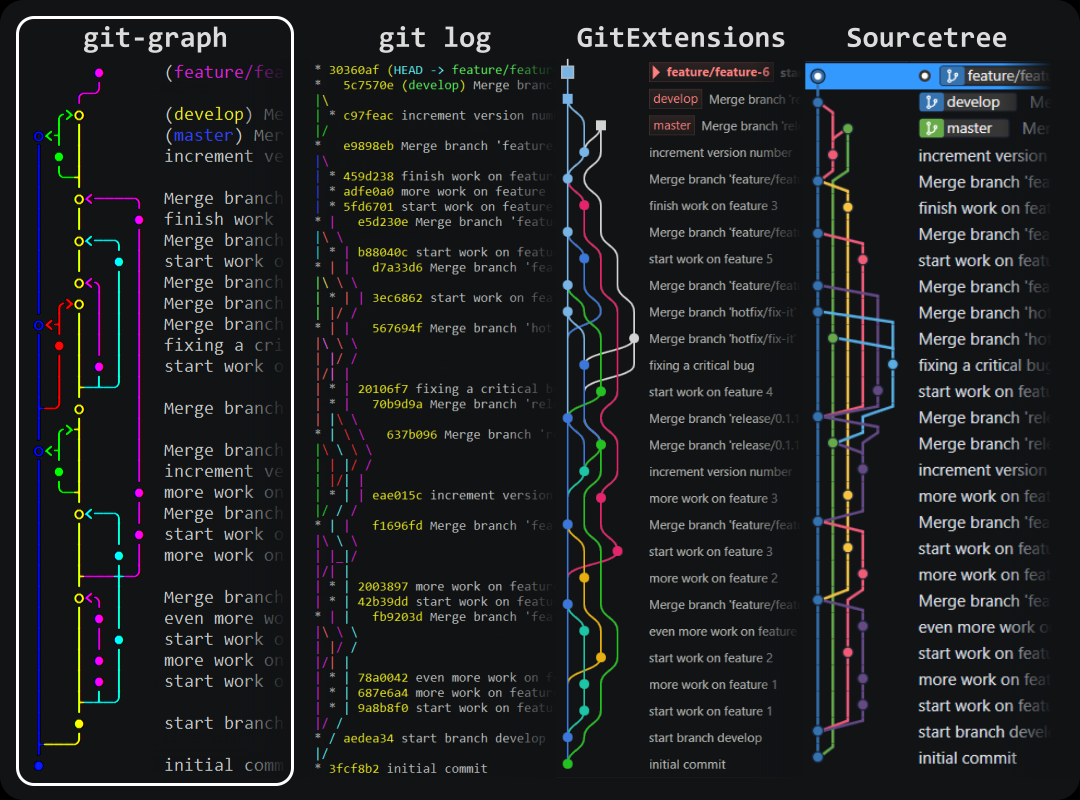
\includegraphics[width=16cm]{assets/git-graph-example.png}
        \caption{Example of Git Graph, Log, Extensions and SourceTree}%
        \label{fig:git-graph}%
    \end{figure}
    \FloatBarrier

    As reiterated throughout our documentation, we use Git and GitHub as our
    version control system, specifically leveraging the power of feature branches
    for effective code management(\autoref{fig:git-graph}).

    \subsubsection{Git and GitHub Integration}
    Our version control process is centered around the use of Git, a distributed
    version control system that enables collaborative development and efficient
    tracking of code changes. GitHub, a web-based hosting service for Git
    repositories, complements our workflow, providing a centralized platform for
    collaboration, code review, and repository management.

    \subsubsection{Feature Branch Workflow}
    The cornerstone of our version control strategy is the utilization of feature
    branches. Feature branches offer a structured approach to development by
    allowing isolated work on specific features or tasks. This ensures that new
    features can be developed, tested, and integrated into the main codebase
    without disrupting the stability of the existing system.

    \subsubsection{Seamless Collaboration}
    By adopting Git and GitHub, our development team benefits from a seamless
    collaboration environment. The platform facilitates easy branching, merging,
    and tracking of code changes. Additionally, GitHub's pull request mechanism
    streamlines the code review process, enabling effective collaboration among
    team members.

    \subsubsection{Committing to Best Practices}
    To maintain a clean and organized version control history, we adhere to best
    practices, including meaningful commit messages and the use of Conventional
    Commits (\autoref{subseq:conventions-sprint-and-task-managment}). This
    commitment to best practices enhances traceability, facilitates code
    maintenance, and ensures a reliable foundation for our development process.

    \section{Development Tools}

    Here you talk about the development tools you've used profoundly. See examples
    belove.

    \subsection{Programming Languages and Frameworks}
    % Discuss the programming languages and frameworks used in your project.
    For the frontend development of our project we used a technology stack that
    includes React, an adopted JavaScript library, TypeScript, a superset of
    JavaScript, and Tailwind CSS, a utility-first CSS framework. For the backend
    development of our project we used Python, a versatile and robust programming
    language, and Django, a high-level web framework.
    \subsection{Version Control}
    % Describe the version control system used and any specific practices.
    In managing our source code, we employed Git, a distributed version control
    system, along with GitHub as our remote repository for seamless collaboration.
    GitHub Desktop offered an intuitive interface for repository management.
    Additionally, we utilized Git-related plugins in Visual Studio Code, including
    GitGraph, enhancing our development environment.

    \subsection{Project Management Tools}
    % Detail the tools used for project management and collaboration.
    Our project management toolkit included Trello for task organization, Figma for
    collaborative design work, and GitHub for version control and code management.
    These platforms collectively facilitated effective communication, streamlined
    workflows, and successful project coordination.

    \subsection{Collaboration and Communication Tools}
    % Discuss tools for team communication and collaboration.
    Our collaboration toolkit featured Trello for seamless task organization,
    GitHub Issues for effective code discussions, and good old in-person
    communication for deeper connections. These tools worked harmoniously to ensure
    clear communication, efficient issue tracking, and genuine team collaboration
    throughout the project lifecycle.

    \subsection{Database Management}
    % Provide insights into the database management system and planning.
    In the realm of database management, we harnessed the power of Django ORM for
    seamless interaction with our database and PostgreSQL for robust data storage.
    This dynamic duo played a vital role in ensuring efficient data handling,
    seamless retrieval, and robust database management throughout our project.

    \subsection{UX/UI Design Tools}
    % Discuss the tools used for designing user experience and interface.
    For crafting our user experience and interface, we turned to Figma and FigJam,
    dynamic tools that fueled our design creativity. Additionally, Shots.so made
    mockup creation a breeze, providing an easy and intuitive platform for bringing
    design concepts to life. Together, these tools formed the backbone of our
    design process, ensuring a seamless and visually appealing user experience.

    \subsection{Code Editors/IDEs}
    % Specify the code editors or integrated development environments.
    In the realm of code, our go-to workstations were VSCode and Neovim. VSCode
    provided a feature-rich integrated development environment, while Neovim
    brought a lightweight and powerful editing experience. These code editors
    served as our creative canvases, empowering us to write efficient, clean, and
    impactful code throughout the project.

    \subsection{Testing and Quality Assurance Tools}
    For checking our frontend's performance, we used Lighthouse integrated with
    Chrome DevTools. Despite some bumps due to unoptimized React code, our website
    scored well – 81 for performance, a perfect 100 for accessibility, 100 for best
    practices, and a solid 90 for SEO. Notably, PWA features weren't available
    during testing, so no score was assigned for Progressive Web App (PWA).

    Additionally, to ensure robust API functionality, we employed Postman,
    conducting comprehensive tests to validate the seamless interaction between the
    frontend and backend components. This dual approach to testing, leveraging both
    Lighthouse and Postman, ensures a thorough evaluation of our system's
    performance and reliability. (\autoref{fig:lighthouse}).

    \begin{figure}[H]
        \centering
        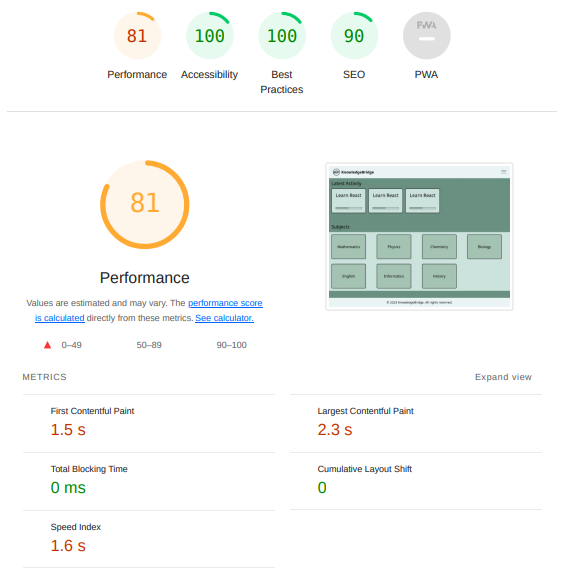
\includegraphics[width=0.8\linewidth]{assets/KnowledgeBridgeLighthouse.png}
        \caption{Lighthouse}
        \label{fig:lighthouse}
    \end{figure}
    \FloatBarrier

    \subsection{Other Tools}
    % Mention any other significant tools used in the development process.
    In our documentation endeavors, we relied on Overleaf for LaTeX-powered
    document collaboration. For visualizing use cases, Visual Paradigm took the
    stage, helping us sketch out comprehensive Use Case diagrams. Together, these
    tools made our documentation journey smooth and efficient.

    \section{The application in action}
    \subsection{UI - realization}

    Here you talk about the process of making the UI of your project (if you have
    one). See an example belove.

    First we created a wire-frame in FigJam, then based on that we created the
    mock-up of the said design. We kept in mind that the users that are going to
    use this page might get frustrated seeing an over complicated website or one
    with too much creativity, thus we made an easy to understand, logical and
    simple design, using one color palette with different shades of the same color.
    We also used generally known icons. \\ \indent After creating an easy to
    understand design with all the useful information about the functionalities we
    created a base front-end project which was the starting point of creating the
    actual website. \\ \indent For the creation of the actual user interface we
    used the powerful combination of React, enhanced by Typescript and styled with
    Tailwind, making it easier to maintain a responsive design. In order to have a
    uniformed style we used components that were easy to use on multiple pages.
    These components made it not only more optimal but also much more comfortable
    the creation of the website. We wanted it to be easy to understand and logical
    for any simple user. \\ \indent We started with the Welcome page as it was the
    easiest. Then the tough part was creating the authentification part. Following
    the design was not the hard part, making it actually work is what made it take
    up a lot of time. Linking the Registration and Login pages to the database via
    the back-end seemed easy at first, but could have been easier have we used an
    already working component. \\ \indent After finally getting the
    authentification to work came the main part of the website, the actual
    must-have. So we started working on the Home page which contains the user's
    latest activities and all the subjects they can access. Same as before, making
    the user interface accordingly to the design was not the hard part, it was the
    linking. Getting back the correct data via request, well it took some time, but
    a lot less than the authentification part. And thus it worked, and with that
    working the Topics, Materials and Material pages was a child's play. Using the
    same components for both the Topics and Materials page was the right choice in
    this case. And for the Material page, there is still thinking to do, but as for
    now it is acceptable the way it looks. \\ \indent Even if it was part of the
    plan, we did not get to actually create the Forum page, however the design is.
    When creating the design we took a look at other pages that maintain either
    Forum pages or pages where people can communicate, by combining these ideas we
    came up with a simple design, where users have the ability to see the latest
    questions, apply filters on them, search for specific ones, save posts, express
    approval or disapproval by liking or commenting, or even ask one themselves.
    This Forum part of the website is meant to connect the users and make it
    possible for them to help one another. \\ \indent There is a lot more to do but
    we are on the same track as the design is and this makes it easier to take just
    a few steps backwards instead of a lot. Having thought about the perspective of
    both the students and the teachers made our work a lot more easy, because we
    once were those students in need of a website like this. And if it was not easy
    for the students, then it must not have been that much easier for the teachers
    either.

    \subsection{Code - realization}

    In this section you talk about the structure of your code, how you've
    implemented the functionalities, etc. You can group by frontend, backend etc.
    functionalities. You may also add screenshots about the code using code
    beautifying tools like \href{https://codeimage.dev/}{CodeImage},
    \href{https://marketplace.visualstudio.com/items?itemName=robertz.code-snapshot}{Code
        Snapshot}, \href{https://snappify.com/}{snappify},
    \href{https://carbon.now.sh/}{carbon} see \autoref{fig:carbon} for an example,
    \href{https://vigowebs.medium.com/awesome-5-tools-to-create-beautiful-images-of-your-code-snippets-2c2df02c6ae2}{etc.}

    \begin{figure}[H]
        \centering
        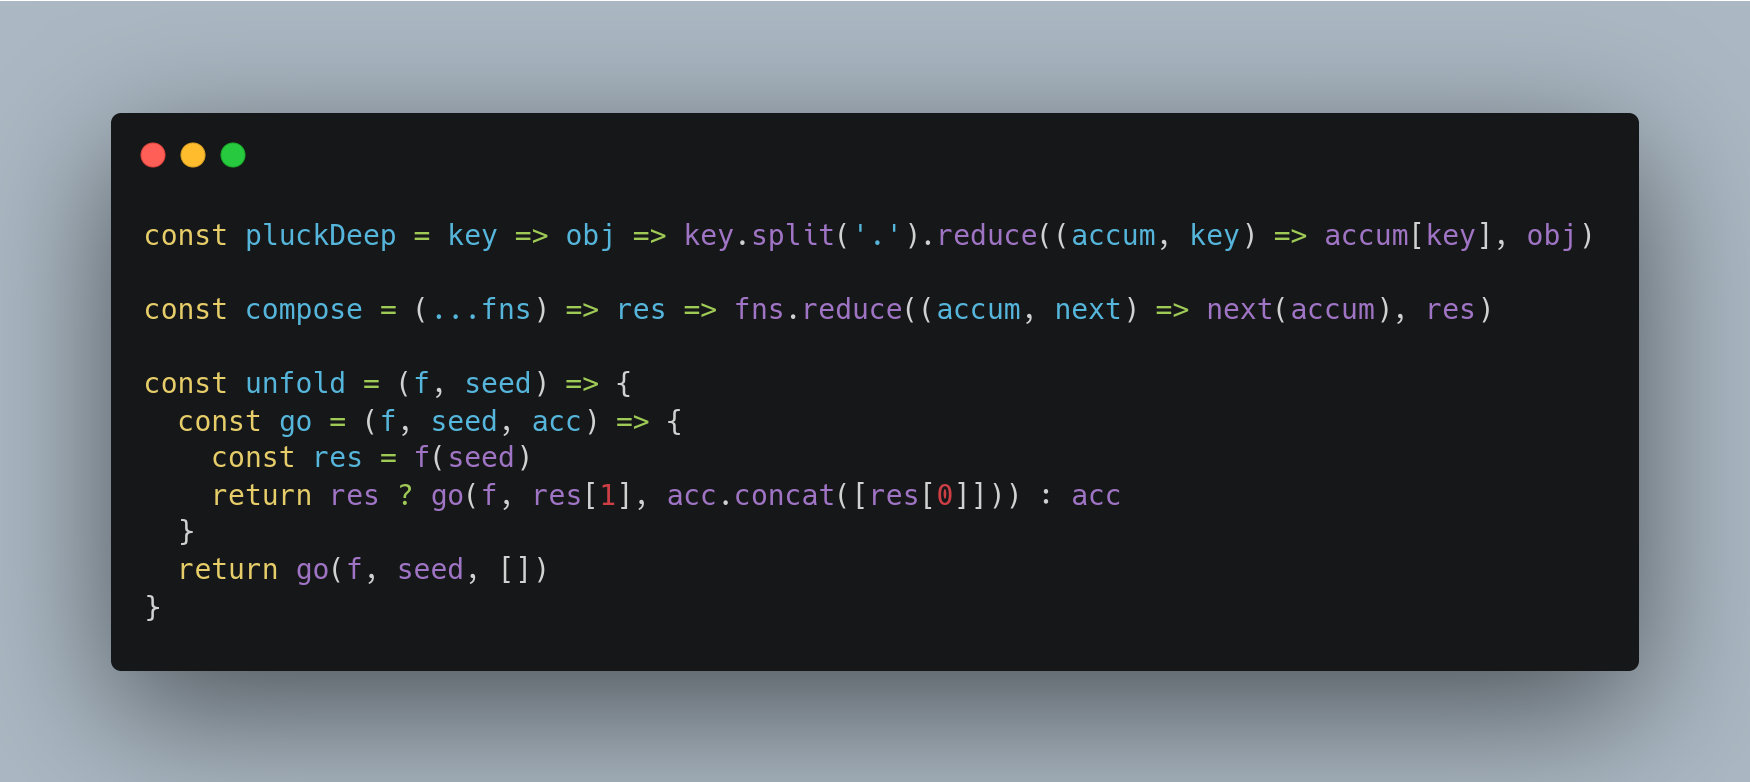
\includegraphics[width=0.9\linewidth]{assets/carbon.png}
        \caption{carbon}
        \label{fig:carbon}
    \end{figure}
    \FloatBarrier

    \section{Summary}

    \textbf{Note:} documentation is not only for the readers it's also for you, so when time
    passes and you don't know something you just have to hit this up and see the
    details.

    Here you summarize the project and the progress of the project creation.

    \subsection{Future improvements}
    Although we had high hopes when starting this project things do not always go
    as planned that is why we have much more elements for this part than we
    originally thought we would have.
    \begin{itemize}
        \item  Before mentioning the original future improvements I would like to mention the
              ones that we wanted to, but unfortunately could not finish.
              \begin{itemize}
                  \item  The very first one is to use a package for the authentification instead of the
                        one we made from scratch.
                  \item  We should also rethink the color palette of the website and use colors that are
                        not too similar to each other, and also make them universal in a way so that we
                        do not have to write it for every component down but rather use a unified dark
                        and light theme on the overall project. \item  Next would be to properly implement the Profile page with all of it's
                        functionalities, including the Settings page.
                  \item  Then comes the Forum page with all of it's functionalities mentioned before.
                        This will be a major task with many smaller components thus it would take a lot
                        more time to make it from scratch thus using a package would help with
                        implementing this part.
                  \item Google authentification should be implemented for an easier authentification
                        system.
              \end{itemize}
        \item Allow me to introduce the originally planned future improvements.
              \begin{itemize}
                  \item Currently the page is in English, but it would be best to make it possible to
                        switch between English, Romanian and Hungarian.
                  \item In high school even though in general we have the same subjects to take exams
                        of, the content of those exams can differ, therefore having major specified
                        topics would help students a lot more than general topics can.
                  \item It is not only high school students that struggle with education and
                        educational materials, middle school and university students are also in the
                        need of educational content that helps with studying, therefore either
                        redesigning this site or making a collection of similar sites would be a great
                        way to help with this problem.
                  \item Another way to improve our site is to directly connect students with teachers
                        by making it possible for them to ask appointments for person-to-person
                        meetings or to directly send them materials to review.
                  \item Having social media accounts would be also great for marketing and interaction.
              \end{itemize}
    \end{itemize}

    \section{Appendix}
    Here you add the appendixes of your documentation, such as big images, long
    code snippets, etc.
    \begin{figure}[H]
        \centering
        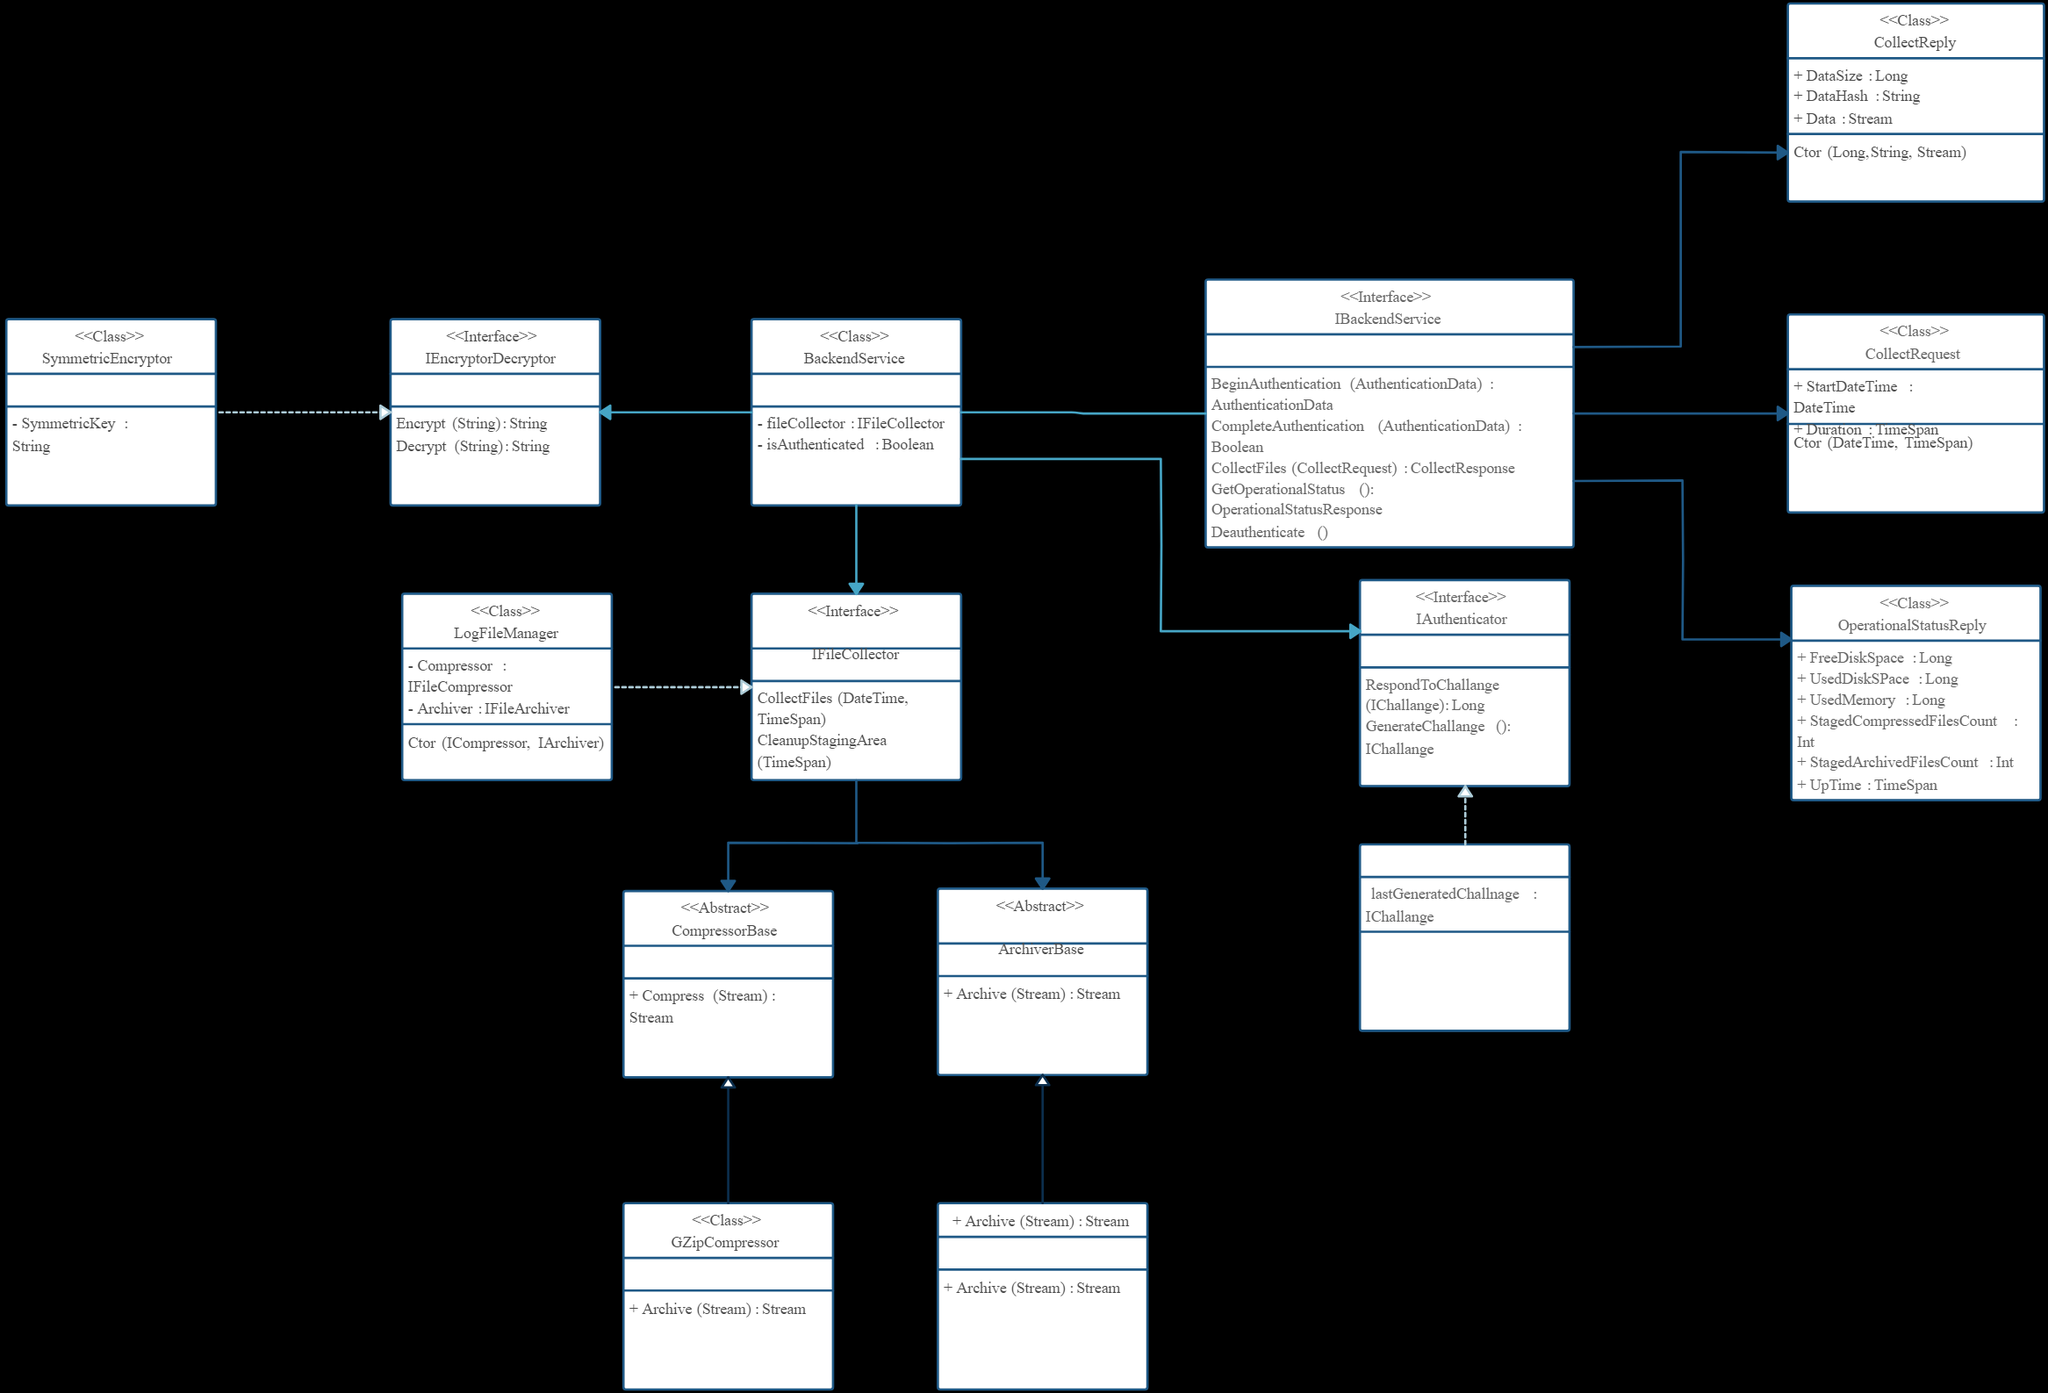
\includegraphics[width=1\linewidth]{assets/backend-uml-example.png}
        \caption{Example UML diagram of the backend}
        \label{fig:backend-uml}
    \end{figure}
    \FloatBarrier

    \begin{figure}[H]
        \centering
        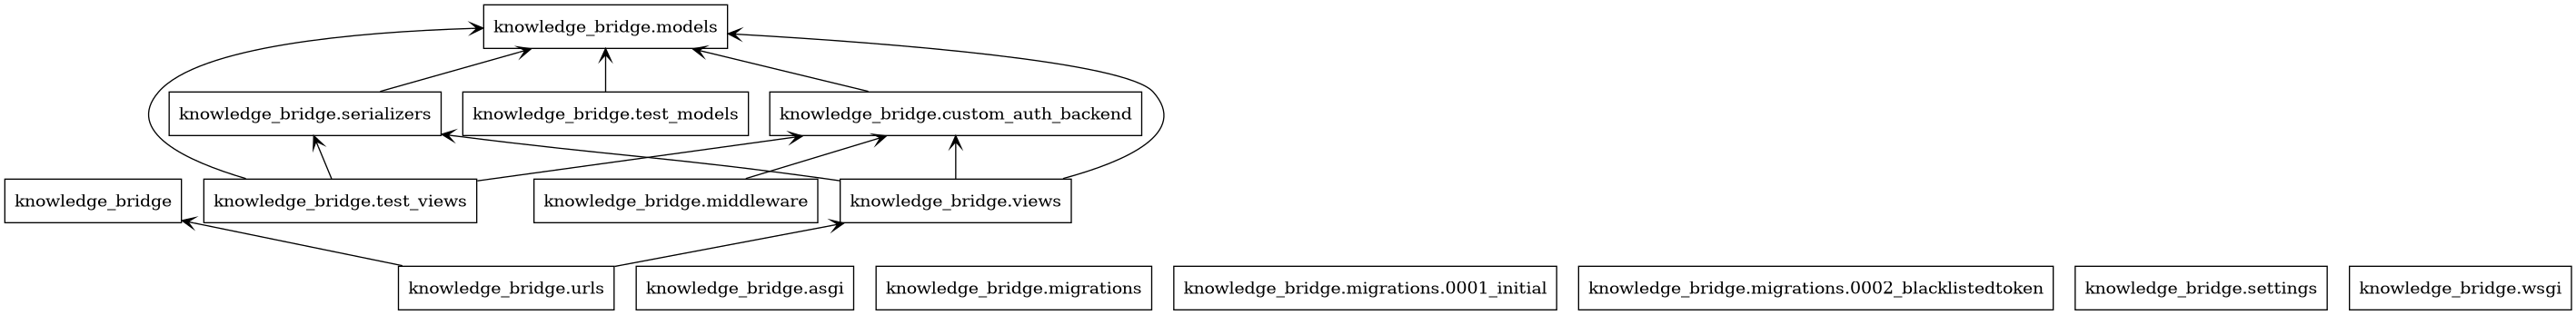
\includegraphics[width=1\linewidth]{assets/KnowledgeBridgePackages.png}
        \caption{Diagram of the backend modules}
        \label{fig:backend-modules}
    \end{figure}
    \FloatBarrier

    %\bibliographystyle{alphabetic}
    %\bibliography{example}
\end{spacing}
\end{document}